%%
%% This is file `mcmthesis-demo.tex',
%% generated with the docstrip utility.
%%
%% The original source files were:
%%
%% mcmthesis.dtx  (with options: `demo')
%%
%% -----------------------------------
%%
%% This is a generated file.
%%
%% Copyright (C)
%%     2010 -- 2015 by Zhaoli Wang
%%     2014 -- 2016 by Liam Huang
%%     2016 -- 2018 by Xuehan Sun
%%
%% This work may be distributed and/or modified under the
%% conditions of the LaTeX Project Public License, either version 1.3
%% of this license or (at your option) any later version.
%%
%% This work has the LPPL maintenance status `maintained'.
%%
%% The Current Maintainer of this work is Xuehan Sun.
%%
\documentclass{mcmthesis}
\mcmsetup{CTeX = false,   % 使用 CTeX 套装时,设置为 true
        tcn = 1920682, problem = B,
        sheet = true, titleinsheet = true, keywordsinsheet = true,
        titlepage = true}
\usepackage{amsmath, amssymb}
\usepackage{mathrsfs}
\usepackage{palatino}
\usepackage{mwe}
\usepackage{graphicx}
\usepackage{subfig}
\usepackage{subcaption}
\usepackage{float}
\usepackage{multirow}
\usepackage{indentfirst}
\usepackage{gensymb}
\usepackage[ruled,lined,commentsnumbered]{algorithm2e}
\usepackage{geometry}
\usepackage{pdfpages}
\usepackage{array}
\usepackage{verbatim}
\usepackage{algorithm}
\geometry{left=2cm,right=2cm,top=2cm,bottom=2cm} %%页边距
\begin{document}
\linespread{0.6} %%行间距
\setlength{\parskip}{0.5\baselineskip} %%段间距
\title{DroneGo: Humanitarian in the Sky to Offer Quick and Adequate Response to Disaster-Stricken Regions}

\date{\today}
	\begin{abstract}

Despite the development of modern science and technology, natural disasters still haunt on people's mind. In 2017, Hurricane Maria, the worst hurricane on record, hit Puerto Rico, causing severe damage and large casualties. Now that natural disasters cannot be killed in the cradle, our central task should be focused on researching new methods to provide timely and adequate response during or after disaster occurs.

To put it into practice, our paper designs a DroneGo disaster response system through which anticipated medical supply demands will be satisfied, if similar disaster scenario takes place like Maria. Within the system, our paper states three basic models to address different subproblems. In the meantime, we implement our models with \emph{a good balance} between two missions-delivery and video reconnaissance. After simulation, we obtain the optimized results of our models and recommend it to HELP, Inc. for future use.

Container Internal Placement Model solves the issue of packing configurations in two aspects. The problem is abstracted into a 3D packaging problem, no matter what object to be packed. We devise an algorithm called \textbf{3D Packaging Judgement}, in which \textbf{Metropolis-Hasting algorithm} is used to provide specific configurations of three containers respectively and alternative solutions for drone cargo bay packing configurations.

Then, we select three locations for three containers based on two main important factors, demand distribution and battery consumption. Demand distribution divide disaster-stricken area into three separated regions,while battery consumption which indicates the max flight radius locates specific location in the three regions. In location selection part, for every drone fleet, which hospital to serve is also determined.

Route Selection Model decides the route through which each drone goes to the hospital and returns, and offers final bay packing configurations. We take total flight distance and max road coverage in to account. The three regions are divided into two kinds, delivery-oriented and reconnaissance-oriented. \textbf{B\'{e}zier Curve} is applied to generate return routes, while \textbf{Simulated Annealing} is employed for routes simulation. After routes are determined, we generate final recommendations for drone payload packing configurations.

The implementation of our model is integrated into each of the three model, we give results and conclusions after explaining our model. While implementing our model, we also survey the literature, google scholar, and other sources, besides the given dataset.

In the end, we make sensitivity analysis and discuss strengths and weaknesses.We also write a memo to the CEO of HELP, Inc., in which we summarize our main outcomes and put forward recommendations.
	
		\begin{keywords}
		3D Packaging Judgement, Metropolis-Hastings algorithm, Analytic Hierarchy Process, B\'{e}zier Curve, Simulated Annealing
		\end{keywords}
	\end{abstract}

\maketitle

\tableofcontents

\newpage

\section{Introduction}

\subsection{Problem Background}

Catastrophic disasters never stops disturbing people's peaceful life, causing many fatalities and huge economic losses. An important method to minimize the effects of terrible disasters is to offer quick and adequate response during or after disasters occur. 

In 2017, Hurricane Maria, the worst hurricane on record to strike the United territory of Puerto Rico, caused severe damages and large casualties, the image of which is presented in Figure \ref{Fig:hurr}(a). The electrical power and cell service outages lasted for months, and many highways and roads across the island were damaged severely. Demands for medical supplies and other medical facilities increased drastically. However, it was barely possible for ground vehicles to access the disaster-stricken region, since roadways were heavily damaged by widespread flood, as shown in Figure \ref{Fig:hurr}(b).

\begin{figure}[htbp]
    \begin{minipage}{0.45\linewidth}
      \centerline{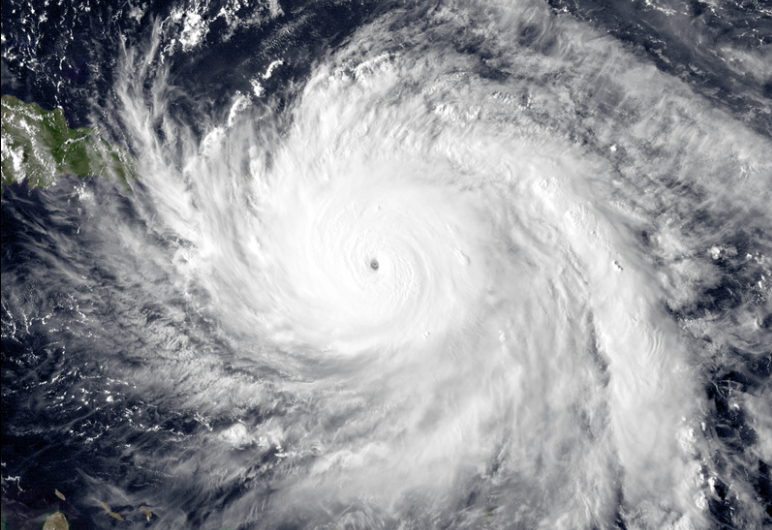
\includegraphics[height = 5.0cm,width=8cm]{figures/hurricanemaria.png}}
      \caption*{(a) Hurricane Maria near peak intensity, moving north towards Puerto Rico, on September 19, 2017.}
    \end{minipage}
    \hspace{0.5in}
    \begin{minipage}{0.45\linewidth}
      \centerline{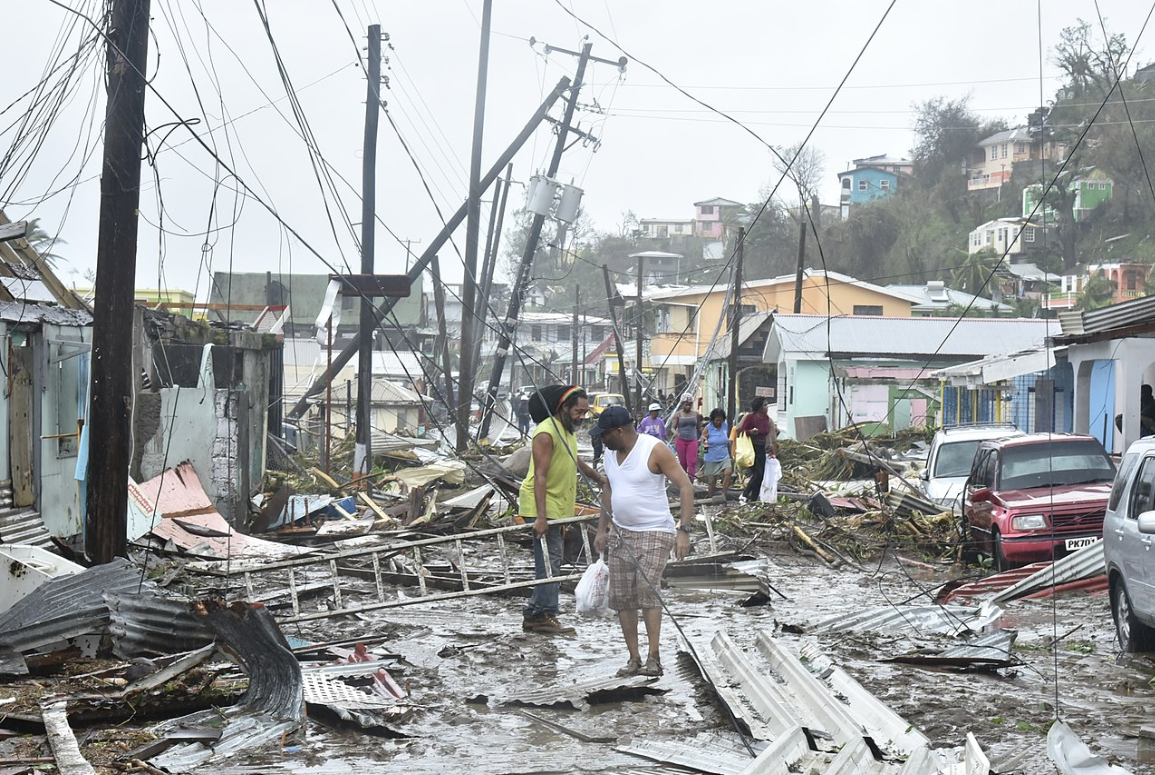
\includegraphics[height=4.9
      cm,width=8cm]{figures/hurricanedamage.png}}
      \caption*{(b) A road is littered with structural debris, damaged vegetation and downed power poles and lines, due to floodings cause by Hurricane Maria}
    \end{minipage}
    \caption{Severe Damages Caused by Hurricane Maria\cite{HurricaneMariaWiki}}
    \label{Fig:hurr}
\end{figure}

Drones are able to perform humanitarian tasks fully and timely, thanks to its means of shipping and fast speed. Its image is shown in Figure \ref{Fig:drsd}. Therefore, a Non-governmental organization(NGO)-HELP, Inc. -aims to promote its disaster response capabilities by applying rotor wing drones to deliver pre-packaged medical supplies and provide high-resolution aerial video reconnaissance, simultaneously or separately. This augments local medical assistance organizations to a great extent.

\begin{figure}[htbp]
    \centering
    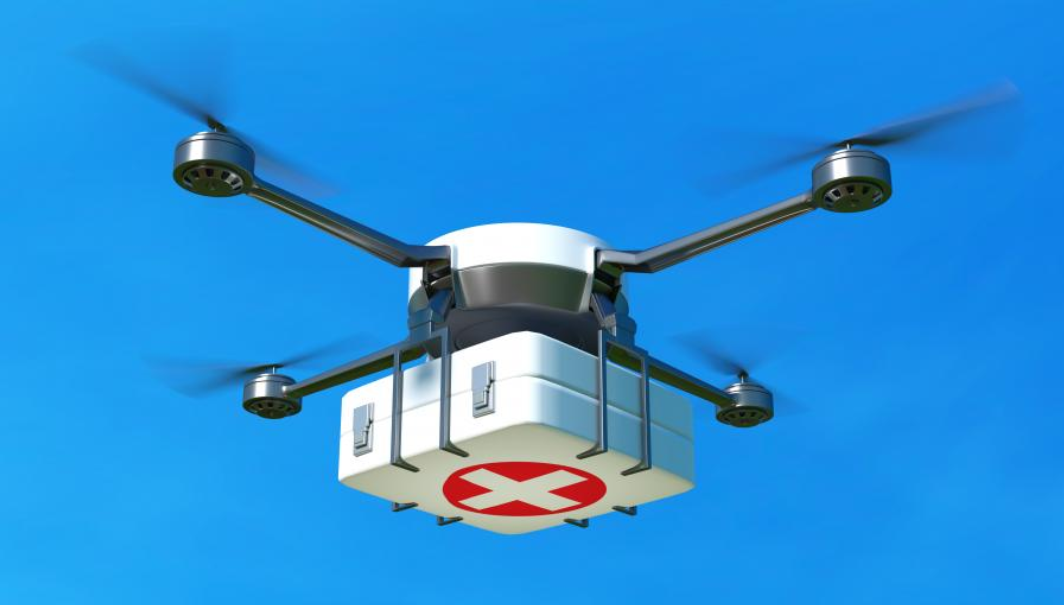
\includegraphics[height=5cm,width=8cm]{figures/uavdisasterrelief.png}
    \caption{Drones for Disaster Relief Purpose}
    \label{Fig:drsd}
\end{figure}

In order to save limited resources and equipment, drone fleets and three locations of containers are restricted, so the response system has to go to great lengths to accomplish the two tasks, \emph{adequate medical supply delivery} and \emph{video reconnaissance}. 

\subsection{Our work}

We take three steps to address the problem. First, we need to solve the packing issue in two aspects, while taking relevant constraints into account. Then, we select three locations for containers, and provides route planning for drone fleet to give consideration to both missions mentioned above. In this paper, we keep a good balance between the two missions, and offer our approach to solve the problem.

In Section \ref{Sec:assu}, we state three basic assumptions. Section \ref{Sec:nome} contains the nomenclature used in our model statement. Section \ref{Sec:stat} offers sufficient details and discussions about our model, and provides results and conclusions of implementing our model at the same time. We further study our model in Section \ref{Sec:mode} by analyzing it in detail. At last, we make some conclusions in Section \ref{Sec:conc}, and submits a memo to the CEO of HELP, Inc. in Section \ref{Sec:memo}.


\section{Assumptions}\label{Sec:assu}
Our model makes the following assumptions:
\begin{enumerate}
	\item HELP, Inc. is able to position each container to the location our model selects, and it is safe and sound to place the container there. This is not influenced by any other factor, such as: flooding or damaged roads.
	\item The take-off and landing process of each drone is ignored. This means both process does not cost power consumption. Additionally, we simplify the speed of the drone to a constant value, which is given in Attachment 2. Thus, total flight time indicates how far a drone can go.
	\item There is often a window phase for the drone fleet to perform tasks. It is common practice that bad weather conditions do not last for a long period, and each drone fleet can meet several days' demands of the hospital for every flight. Therefore, it is reasonable to assume like this.
\end{enumerate}


\section{Nomenclature}\label{Sec:nome}
In this paper, we use the nomenclature in Table \ref{Tab:nome} to describe our model. Other symbols that are used only once or twice will be described later in the context.
\begin{table}[htbp]
    \centering
    \caption{Nomenclature}
    \label{Tab:nome}
    \linespread{1.5}
    \begin{tabular}{c c}
\toprule
    	Symbol & Definition\\
\midrule
	$C_i$ & The \emph{i}th container, \emph{i}=1,2,3\\
	$D_{i,j}$ & The \emph{j}th drone of the \emph{i}th container,\emph{j} follows the order of A to H\\
	$B_{i,j}$ & The cargo bay of $D_{i,j}$\\
	$P_{i,j,k}$ & The \emph{k}th medical package of $B_{i,j}$\\
	$L,W,H$ & The length, width, and height of a standard ISO container\\
	$l_m,w_m,h_m$ & The length, width, and height of the \emph{m}th object to be placed into the container\\
	$M(x,y)$ & The importance distribution of medical demand for each map point $(x,y)$\\
    $n_{s,t}$ & The quantity demand of the \emph{t}th medical package of the \emph{s}th hospital\\
    $R$ & The set of point on roads\\
    $I_R(x, y)$ & The road indicator function \\ 
    $S_i$ & The reachable road area of the $i$th container \\
    $N_{D,i}$ & The number of deployed drones in the $i$th container\\
	
\bottomrule
    \end{tabular}
\end{table}


\section{Statement of our Model}\label{Sec:stat}

In this section, we will discuss all details about our model. The model take many factors into consideration, based on the given dataset and online researching of other important things. To begin with, we first put forward our model of packing configurations of three containers and drone payload. Afterwards, three locations are selected to position three containers respectively. Finally, we plan the detailed routes of our drone fleets. The model keeps a great balance between delivery and video reconnaissance\cite{IEEEConference}. The complete diagram is vividly shown in Figure \ref{Fig:flo}.

\begin{figure}[htbp]
    \centering
    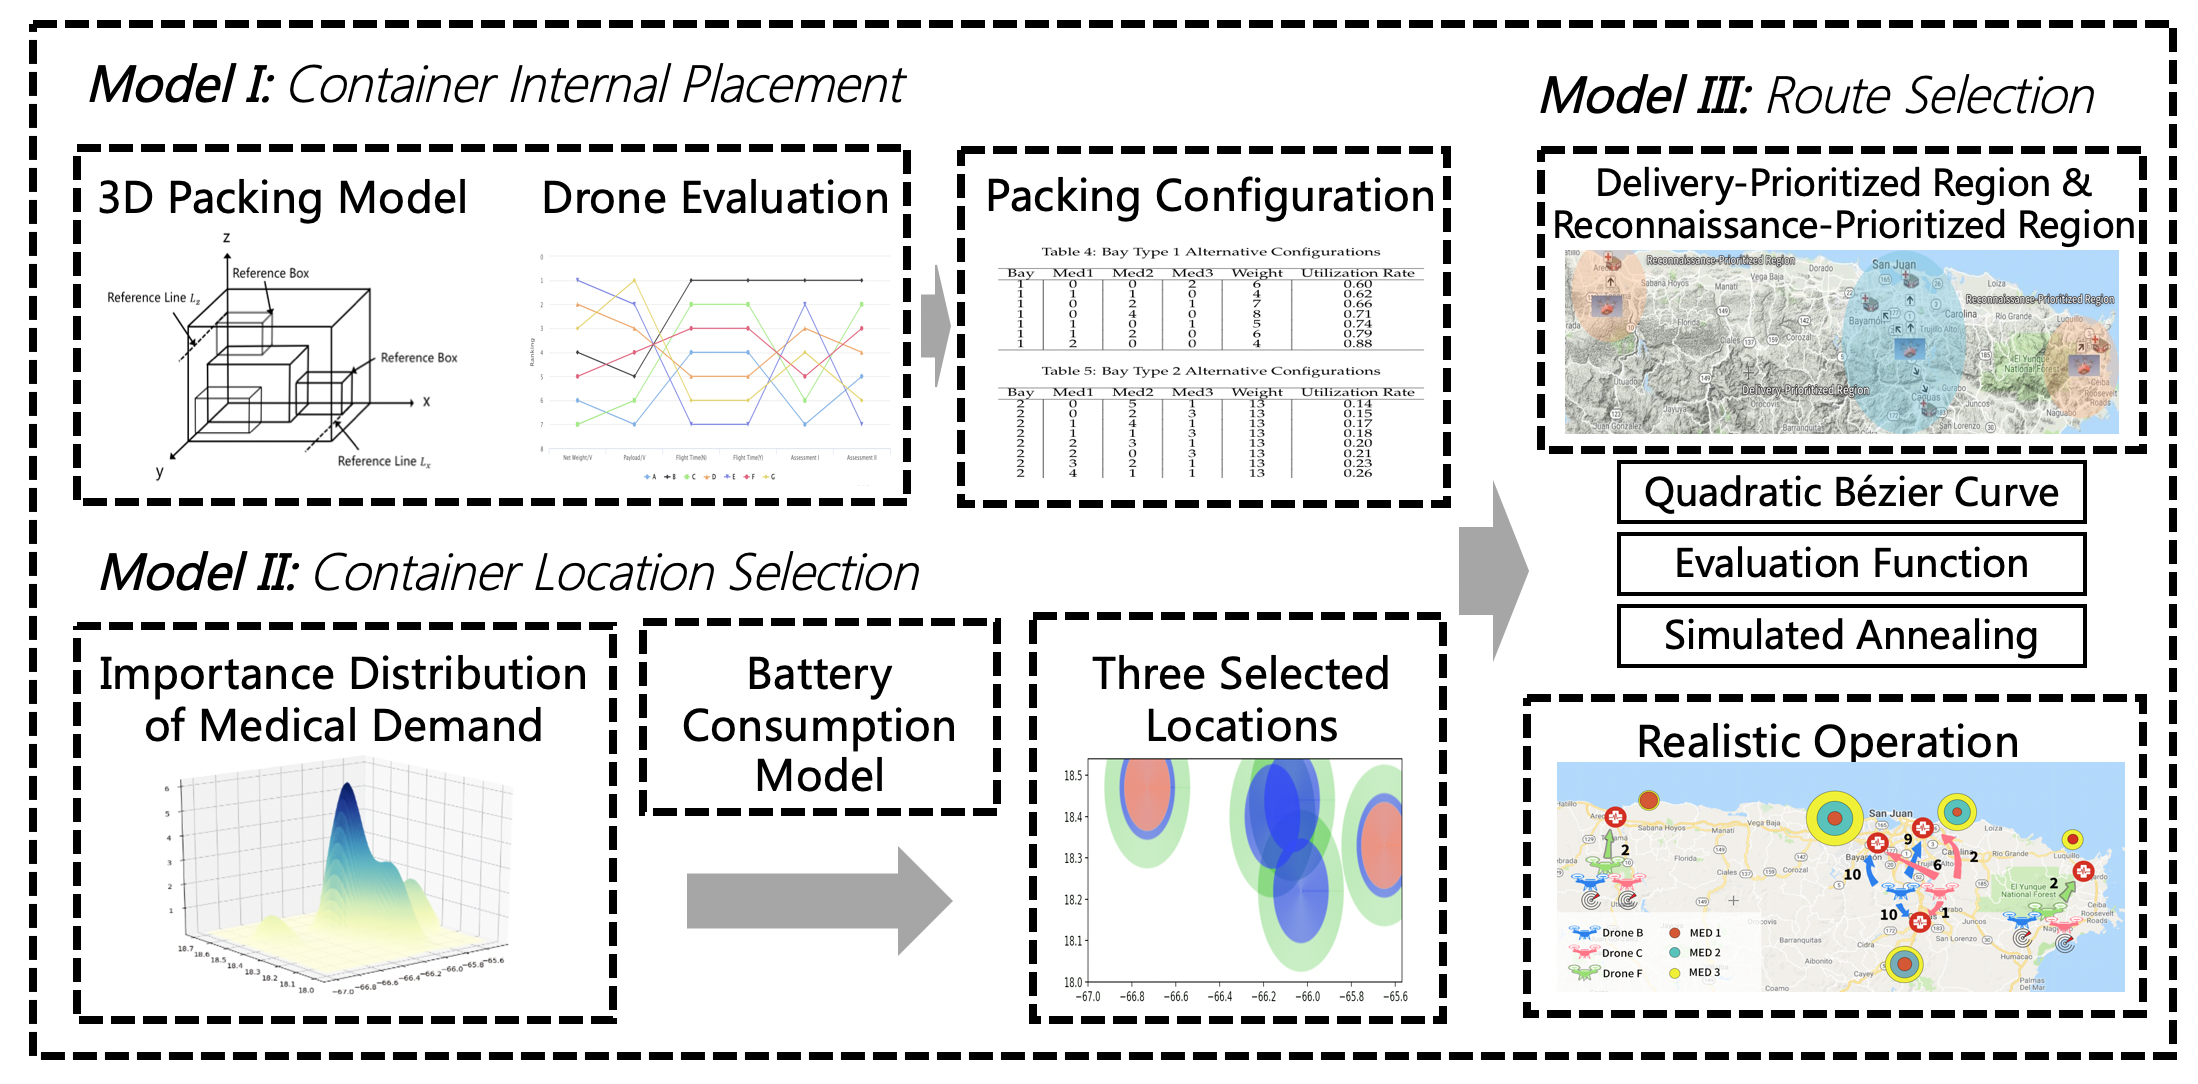
\includegraphics[width=17cm]{figures/flowchart.png}
    \caption{The Entire Diagram of Our Three Models}
    \label{Fig:flo}
\end{figure}

\subsection{Container Internal Placement Model}

Container Internal Placement Model gives solutions to \emph{which and how} drones and their cargo bays inside the container are configured, as well as \emph{which and how} medical packages inside the cargo bay are configured. The two configurations are quite similar, so they \emph{share the same Algorithm \ref{Algo:3dpa}} in our model.

We first solve the problem of \emph{how}, after which we come up with drone evaluation to address the problem of \emph{“which”}.

Our model gives \emph{determined} configurations of drones and their bays for the three shipping containers, and provides \emph{alternative} configurations of medical packages that make good use of drone cargo bay. However, medical supply demands from the six local hospitals should be satisfied. Therefore, we will select the most proper cargo bay configuration in our implement part in Section \ref{Subsub:real}.

\subsubsection{The Structure of Container and Cargo Bay}
Each container is composed of different combinations of a drone and its cargo bay, or simply a drone itself, while every cargo bay consists of different combinations of three medical packages. The relationship among them is clearly depicted in the tree diagram below in Figure \ref{Fig:ther}.

\begin{figure}[htbp]
    \centering
    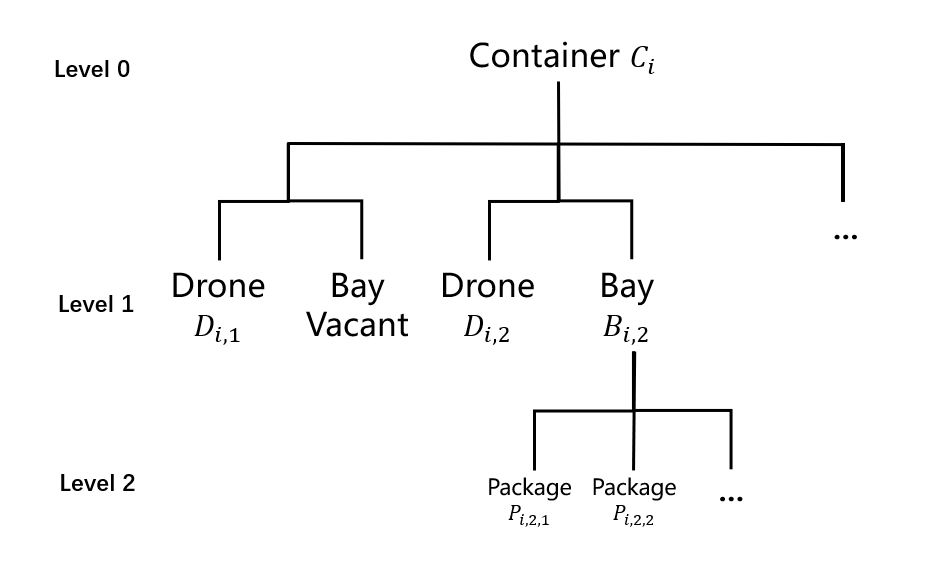
\includegraphics[height=6cm,width=10cm]{figures/relationship2.png}
    \caption{The Relationship Among Container, Drone and Its Bay, and Medical Package}
    \label{Fig:ther}
\end{figure}

Apart from given size(length, width, and height) of a standard container and two kinds of cargo bays that must be complied with, it is clear that the type of cargo bay relies on its drone, and the number of cargo bays \emph{less than} that of drones. This provides restrictions for Section \ref{Subsub:cont}.

\subsubsection{3D Packaging Judgement}\label{Sec:3dpa}

\paragraph{Inspiration}When building up a wall, people generally place \emph{a brick for reference} in the first place. Then, people set the height of \emph{the brick for reference} as a benchmark, and stipulate the height of each object placed-inside less than the benchmark. The benchmark can be heightened, only when no object can be placed inside.

\paragraph{Operation}During our three-dimension packing process, similar "reference brick" is introduced in x-axis and z-axis directions to guide \emph{the container-loading and drone cargo bay-loading course}. For simplicity, both drones and cargo bays to be put inside the container are called objects. We use points where another object can be placed or \emph{available points} to describe and find where the next object can be placed inside. For each object put into the container, it occupies a single available point and generates three similar points. The operation is derived from \textbf{the Greedy Algorithm} and \textbf{the Heuristic Algorithm}, but what makes the operation distinctive is that it does not need to fit in with a certain structure. This makes our loading process quite flexible.

\noindent As mentioned above, we are going to put either a drone and a drone's cargo bay into a box. Suppose we have boxes series $\{b_1,b_2,\dots,b_n\}$. At the beginning, the 1st box $b_1$ can be put at $(0,0,0)$. Afterwards, $b_2$ has three available points $(l_1,0,0),(0,w_1,0),(0,0,h_1)$. Suppose the 2nd box chooses $(l_1,0,0)$, we delete the available point $(l_1,0,0)$ and add $(l_1+l_2,0,0),(l_1,w_2,0),(l_1,0,h_2)$ to the set of available points.

\noindent As for reference line, we select the reference line $L_z$ and the reference line $L_x$, both parallel to axis $y$, as shown in Figure \ref{Fig:pack}(b). We sort the objects attached to available points by $y$ from small to large. If $y$ is equal, sort by $x$ from small to large. If $x,y$ are equal, sort by $z$. Suppose we are trying to put an object to available point. Before placing, the container $C_i$ cannot overlap in any part. Besides, the object$(\tau_m)$ should satisfy the equation: $z+h_m\leq L_z, x+l_m\leq L_x$. When the first feasible available point is found, we attach the object to it. If there is not any feasible points, we conduct the following steps: (1) If $L_x< L$, then we raise the reference line $L_x$. (2) Otherwise, we raise the reference line $L_z$. After raising both reference lines, if the object still can't be put in, we no longer consider the object.

\begin{figure}[htb]
    \begin{minipage}{0.48\linewidth}
    \centerline{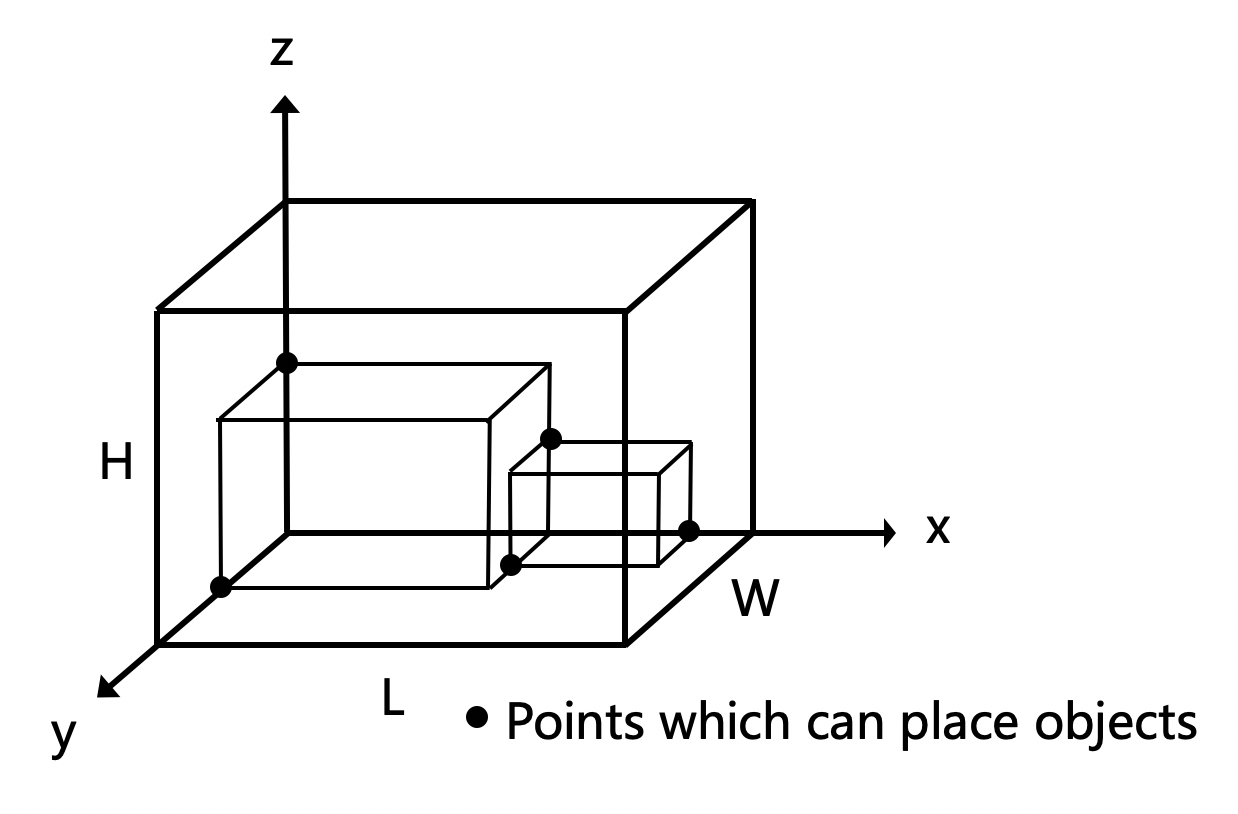
\includegraphics[width=7.0cm]{figures/availablepoints2.png}}
    \centerline{(a) Available Points}
    \end{minipage}
    \begin{minipage}{0.48\linewidth}
    \centerline{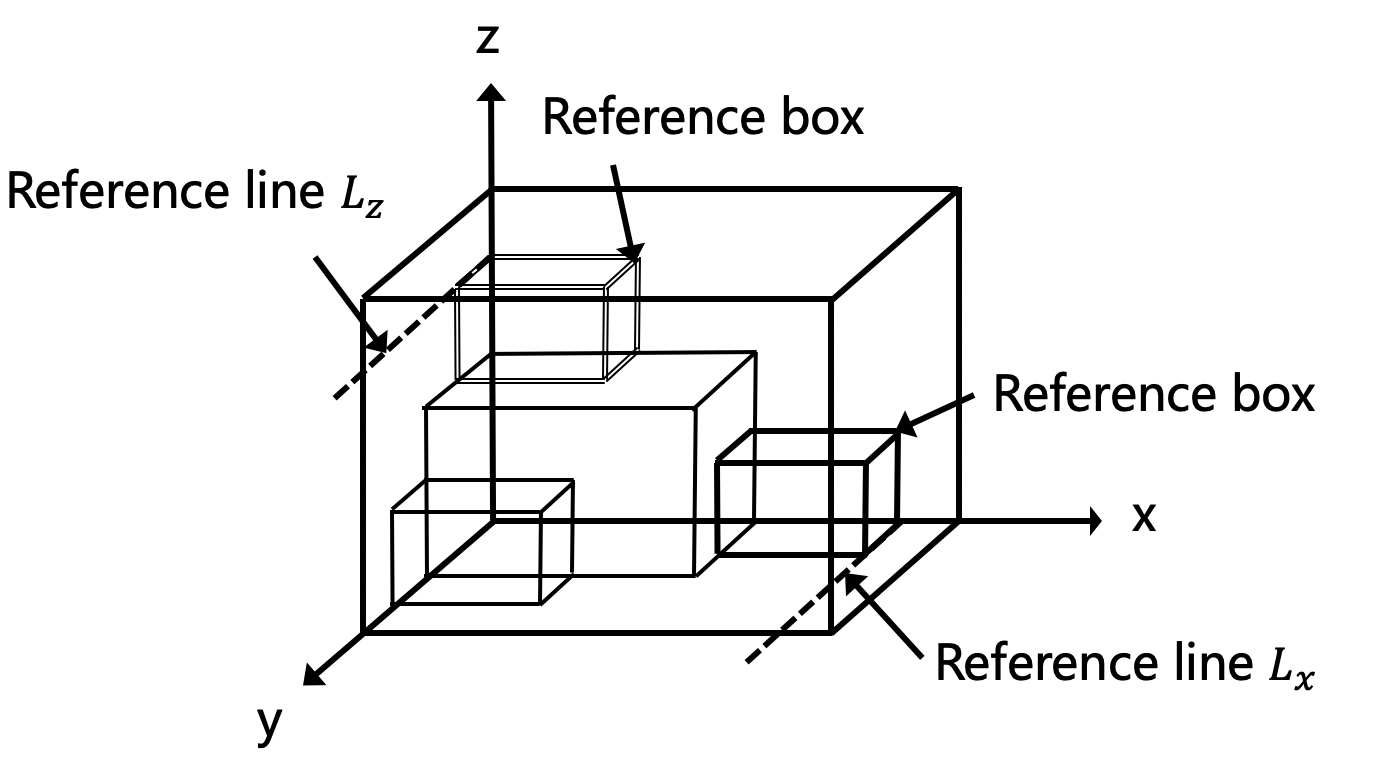
\includegraphics[width=7cm]{figures/referenceline.png}}
    \centerline{(b) Horizontal and Vertical Line}
    \end{minipage}
    \caption{Two Major Steps of 3D Packaging Judgment}
    \label{Fig:pack}
\end{figure}

After researching, we devise an algorithm called \textbf{3D Packaging Judgement}, shown in Algorithm \ref{Algo:3dpa} \cite{Packing}. The time complexity of the algorithm is $O(n^3)$. In order to simplify the problem, we assume that the object(drone or its cargo bay) cannot rotate horizontally. In rotation cases concerning the axis $z$, rotation should not be taken into account at all, since medical supplies consist of some fragile and delicate equipment. Once damaged, its utility reduces a lot, eventually causing unnecessary losses that outweigh space saved.

\begin{algorithm}[h]
\caption{3D Packaging Judgement}\label{Algo:3dpa}
\KwIn{$B=\{b_1,b_2,\dots,b_n\}$}  
\KwOut{True or False}  
$I\leftarrow\{(0,0,0)\}, L_z \leftarrow 0, L_x 
\leftarrow 0,count\leftarrow 0$\;
  
\For{$i$ from 1 to $n$}  
{  
    $flag \leftarrow$ False\;
    
    \ForEach{$(x,y,z)\in I$}
    {
        \If{$b_i$ can be put into position $(x,y,z)$ and $x+ l_i\leq L_x, z+ h_i\leq L_z$}
        {
            $flag \leftarrow$ True, break}
        \If{$flag$ = False}
        {
            \If{$L_x=0$ or $L_x=L$}
            {
                \If{$b_i$ can be put into position $(0,0,L_z)$}
                {
                    $x\leftarrow 0,y\leftarrow 0,z\leftarrow L_z,flag\leftarrow$True$,L_z\leftarrow L_z+h_i,L_x\leftarrow l_i$\;
                }
                \ElseIf{$L_z<H$}
                {
                    $L_z\leftarrow H,L_x\leftarrow L,i\leftarrow i-1$\;
                }
            }
            \Else
            {
                \ForEach{$(x,y,z)\in I$ which $x=L_x,y=0$}
                {
                    \If{$b_i$ can be put into position $(0,0,L_z)$ and $z+h_i\leq L_z$}
                    {
                        $flag\leftarrow$ True$,L_x\leftarrow L_x+l_i$, break\;
                    }
                }
                \If{$flag=$ False}
                {
                    $L_x\leftarrow L$, $i\leftarrow i-1$\;
                }
            }
            
        }
        \If{$flag=$ True}
        {
            Put $b_i$ into position $(x,y,z)$, $I=I/\{(x,y,z)\}$, move $b_i$ along the X, Y, Z axis coordinate reduction direction and get $(x',y',z')$, $I=I\cup \{(x'+l_i,y',z'),(x',y'+w_i,z'),(x',y',z'+h_i)\}$\;
            $count \leftarrow count + 1$ 
        }
    }
}
\Return{$count=n$}  
\end{algorithm}  

\newpage
Although the rotation-included program is not realizable during our modeling time, we do design the whole process of it, which can be clearly seen in Appendix \ref{App:rota}. Provided that enough time is given, the results of the program can be surely obtained.

\clearpage

\subsubsection{Drone Evaluation System}

Since the two missions - \emph{medical supply delivery} and \emph{video reconnaissance} require different capabilities of drones, our drone evaluation system provides two assessment for each task accordingly. When it comes to the delivery mission, drones' max flight distance and shipping ability are both taken into account, while we only consider max flight distance for reconnaissance mission. 

Assessment I is relevant to four determining factors, net weight per volume, max payload capability per volume, flight time with no cargo, and flight time with full cargo. Flight time with full cargo is related to battery conditions, which our model will give a detailed discussion in Section \ref{Subsub:batt}. Therefore, the Assessment I equation is can be stated as follows in Equation \eqref{Equ:ass1}.

\begin{equation}\label{Equ:ass1}
    A_1 = c_{11}\times\frac{N_i}{V_i} + c_{12}\times\frac{L_i}{V_i^{'}} + c_{12}\times\frac{F_{1,i}}{\max  \left(F_{1,i}\right)} + c_{14}\times\frac{F_{2,i}}{\max \left(F_{2,i}\right)}
\end{equation}

Similarly, Assessment II is relevant to flight time with no cargo, and flight time with full cargo. It is stated in Equation \eqref{Equ:ass2}.

\begin{equation}\label{Equ:ass2}
    A_2 = c_{21}\times\frac{F_{1,i}}{\max  \left(F_{1,i}\right)} + c_{22}\times\frac{F_{2,i}}{\max \left(F_{2,i}\right)}
\end{equation}

where:
\begin{itemize}
    \item $N_i$ is the net weight of the \emph{i}th drone;
    \item $V_i$ is the volume of the \emph{i}th drone;
    \item $L_i$ is the max payload capacity of the \emph{i}th drone;
    \item $V_i^{'}$ is the volume of the \emph{i}th drone and its cargo bay;
    \item $F_{1,i}$ is flight time with no cargo of the \emph{i}th drone;
    \item $F_{2,i}$ is flight time with full cargo of the \emph{i}th drone;
    \item $c_{m,n}$ is the weight of each term.
\end{itemize}

The \textbf{Analytic Hierarchy Process(AHP)} is a structured technique for organizing and analyzing complex decisions, based on mathematics and psychology. We use AHP to determine $c_{1,k}$ coefficients, shown in Table \ref{Tab:AHP}. We apply importance proportion to determine $c_{21}$ and ${c_{22}}$. One thing is clear that flight time matters a lot, as it decides whether a local hospital can be supported.

\begin{table}[h]
    \centering
    \caption{AHP production}
    \label{Tab:AHP}
    \begin{tabular}{c c}
\hline
    	Coefficient & Weight\\
\hline
	$c_{11}$ & 0.2292\\
	$c_{12}$ & 0.2278\\
	$c_{13}$ & 0.1119\\
	$c_{14}$ & 0.4221\\
\hline
    \end{tabular}
\end{table}

Afterwards, we use the two formula to evaluate different types of drones, and normalize them by dividing each by the largest value, which is clearly indicated in Figure \ref{Fig:asse}.


\begin{figure}[htbp]
    \centering
    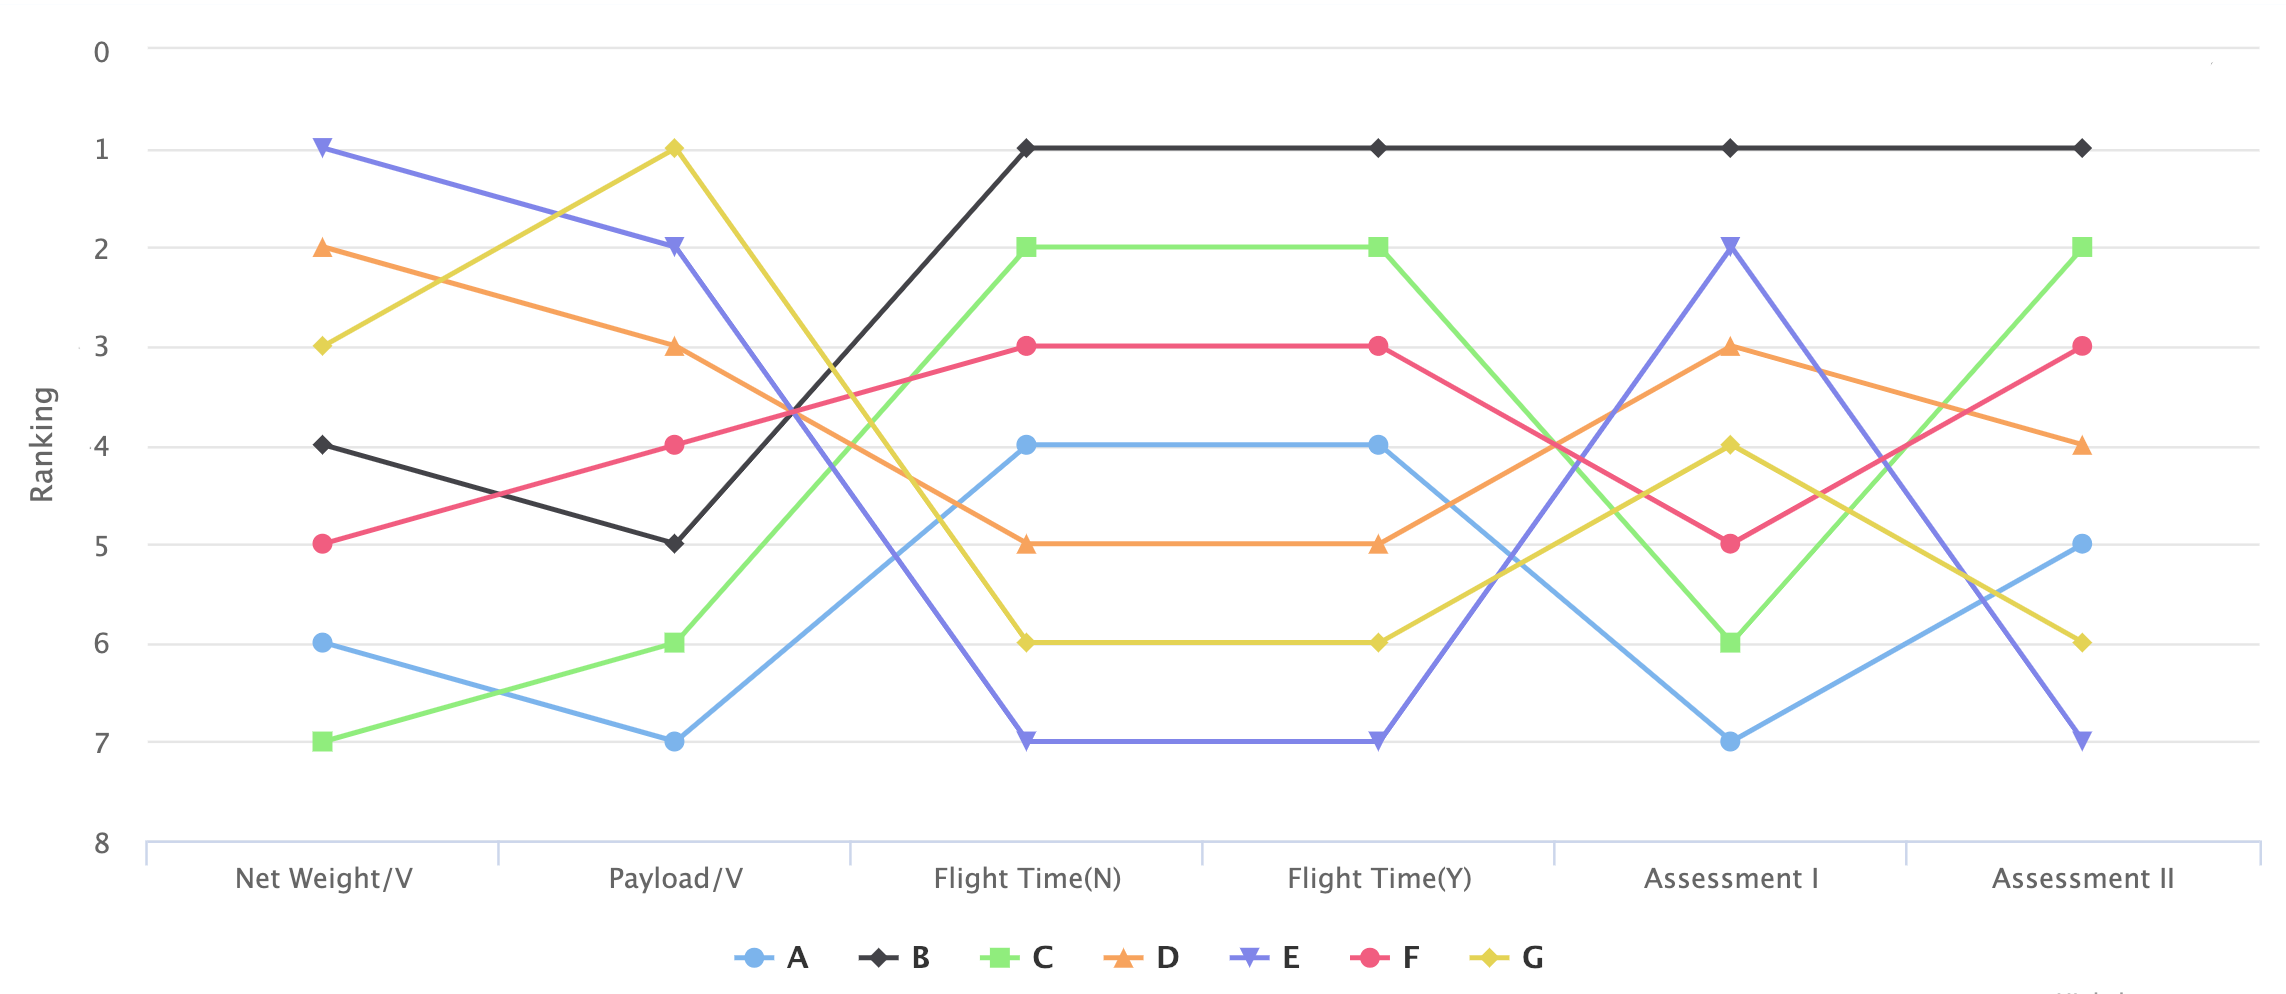
\includegraphics[width=14cm,height=6cm]{figures/radarassessment.png}
    \caption{Assessment I and II Chart of Different Drones}
    \label{Fig:asse}
\end{figure}

\paragraph{Conclusions}For \emph{delivery mission}, we select Drone B and Drone C; for \emph{reconnaissance} mission, we select Drone B, Drone C, and either Drone F or Drone G.

\subsubsection{Container Packing Configuration}\label{Subsub:cont}

If we have one group of a drone and its cargo bay, or simply a drone, we can make judgment whether it is feasible to be placed inside the container through Section \ref{Sec:3dpa}. Clearly, it is unwise to enumerate all possible conditions. Thus, we choose to apply \textbf{Metropolis-Hastings algorithm(MHA)} \cite{MetropolisHastingsAlgorithm} to obtain the optimized outcomes.

\begin{enumerate}[STEP 1]
    \item Generate a random selection sequence $\theta_k=\{N_{k,1},N_{k,2},\dots,N_{k,n}\}$, where $N_{k,j}$ is the number of $j$th drone. 
    \item Generate $\theta$. Our generation rule is that there is a chance of $p$ to randomly generate new $\theta$, and a probability of $(1-p)$ : $\theta\leftarrow \theta_k + \varepsilon, \varepsilon \sim N(0,\sigma)$ . If $\theta$ is not feasible, as verified by Section \ref{Sec:3dpa}, we regenerate it.
    \item We have a chance of $\alpha$ to accept the newly-generated $\theta$ as $\theta_{k+1}$. Here, $\alpha=\min(1, SU(\theta)/SU(\theta_{k}))$, where $SU(\theta)$ is the space utilization rate of $\theta$.
\end{enumerate}

Therefore, for $N(=N_{k,1}+N_{k,2}+\dots+N_{k,n})$, after $N$ is determined, we can get reasonable outcomes. 

\paragraph{Drone Fleets' Results}For \emph{delivery-oriented mission}, we are prefer to configure twenty-nine Drone Bs all with bays and nine Drone Cs all with their bays, too. Table \label{Tab:twok} clearly presents our outcomes; for \emph{reconnaissance-oriented} mission, we are tend to configure twenty Drone Bs with no bay, nine Drone Cs without any bay, and two Drone Fs all with bays

\begin{table}[h]
    \centering
    \caption{Two Kinds of Container Packing Configuration or Drone Fleets}
    \label{Tab:twok}
    \begin{tabular}{c c c|c c c}
\hline
         \, & Drone Fleet I & \, & \,& Drone Fleet II & \,\\
    	Drone & Bay & Quantity & Drone & Bay & Quantity\\
\hline
	$B$ & $\surd$ & 29 & $B$ & $\times$ & 20\\
	$C$ & $\surd$ &  9 & $C$ & $\times$ &  9\\
	 \, &    \,   &  \,& $F$ & $\surd$  &  2\\
\hline
    \end{tabular}
\end{table}


\subsubsection{Drone Payload Packing Configuration}

Similar to the methods used in Section \ref{Subsub:cont}, we get different configurations of medical packages in a drone cargo bay. Our configuration offers different combinations of medical packages, and the combination can be chosen according to local hospital demands. 

\paragraph{Results}Our model produces seven alternative configurations for cargo bay type 1, and twenty-eight potential configurations for cargo bay type 2. The average utilization rate for bay type 1 is $71.4\%$, while it is $21\%$ for bay type 2. The utilization rate is such low for bay type, because bay type 2 is much larger than bay type 1, and there exists max payload capability restrictions. The entire options are listed in the Appendix \ref{App:alte}.

After discussion in \ref{Sec:cont}, we will screen through these data and give out recommendations. At this step, we only provide alternative solutions for max utilization rate. After taking hospitals' demands and locations into consideration, alternative solutions will be narrowed down to recommendations.

\subsection{Container Location Selection Model}\label{Sec:cont}

In this section, our model identifies the best locations on Puerto Rico to position three cargo containers. First, we give the Importance Distribution of Medical Demand to indicate three isolated regions. Then, based on the speed and max flight time full cargo of each drone, we obtain a max flight radius for each drone. After that, we finally get three container locations.

\subsubsection{Importance Distribution of Medical Demand}

In this part, we give the Importance Distribution of Medical Demand to divide Puerto Rico into several demand-related regions. Relying on the location(longitude and latitude) of five hospitals and their varied demands for three medical packages, as presented in Figure \ref{Fig:hosp}, we generate the formula of $M(x,y)$. Only land areas are considered, and we make map points off land zero, since it is impossible to locate containers on sea. From Figure \ref{Fig:impo}, we can clearly see three peaks, and this divides five hospital into three separated parts. In each of three part, there is a container location, in which its drone fleet \emph{only serves} hospitals in this separated part.

\begin{figure}[htbp]
    \centering
    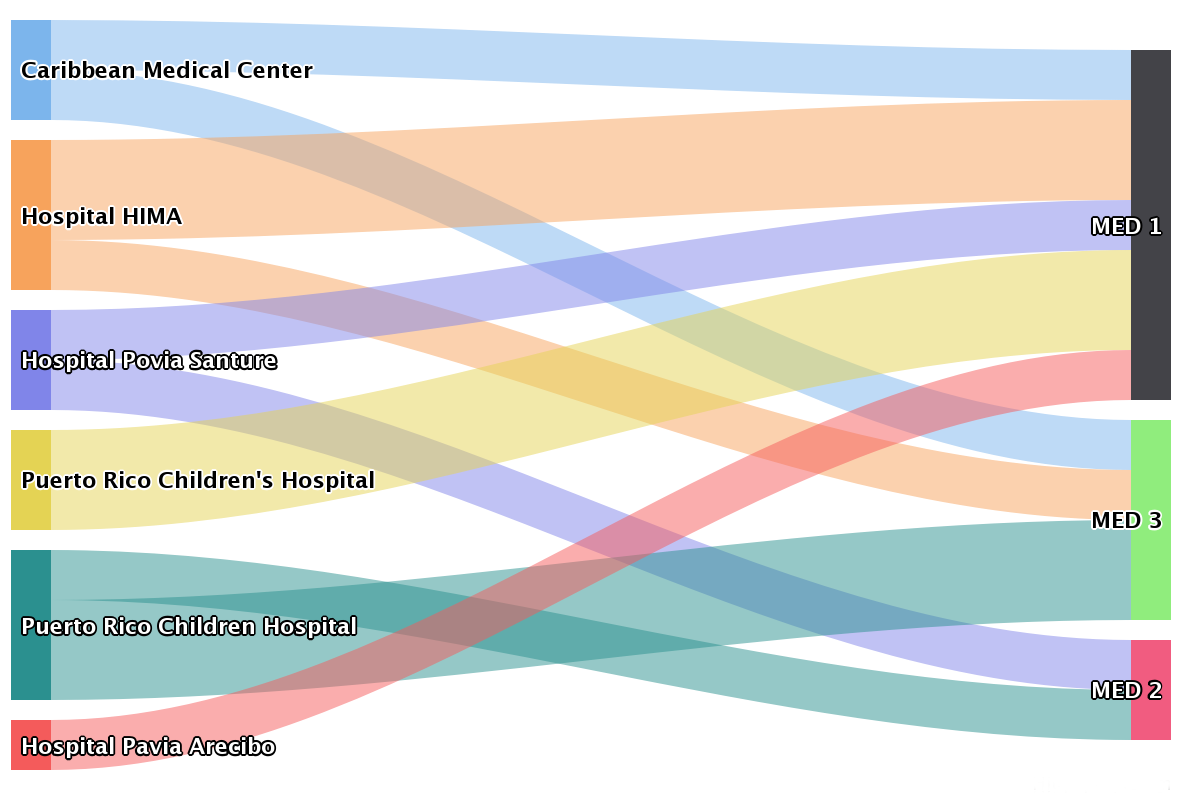
\includegraphics[height=6cm,width=10cm]{figures/hospitalchart.png}
    \caption{Five Hospital Different Demands for Different Medical Packages}
    \label{Fig:hosp}
\end{figure}

We use latitude($H_{s,x}$) and longitude ($H_{s,y}$) of the \emph{s}th hospital location, and latitude($x$) and longitude($y$) of each map point to calculate the straight-line distance between them, presented in Equation \eqref{Equ:dist}.

\begin{equation}\label{Equ:dist}
       d_s = \left(\frac{\pi R_0}{180} \right)\times \mathrm{arccos}[\sin{H_{s,x}}\sin{x}\cos{(H_{s,y}-y)}+\cos{H_{s,x}}\cos{x}]\\
\end{equation}
where $R_0$ is the radium of earth.

$M(x,y)$ relies on the distance $d_s$.
\begin{equation}\label{Equ:medi}
    M(x,y) = \sum_{s=1}^5 \sum_{t=1}^3 n_{s,t} e^{-\frac{d_s^2}{2\sigma^{2}}}
\end{equation}

\begin{figure}[htbp]
    \centering
    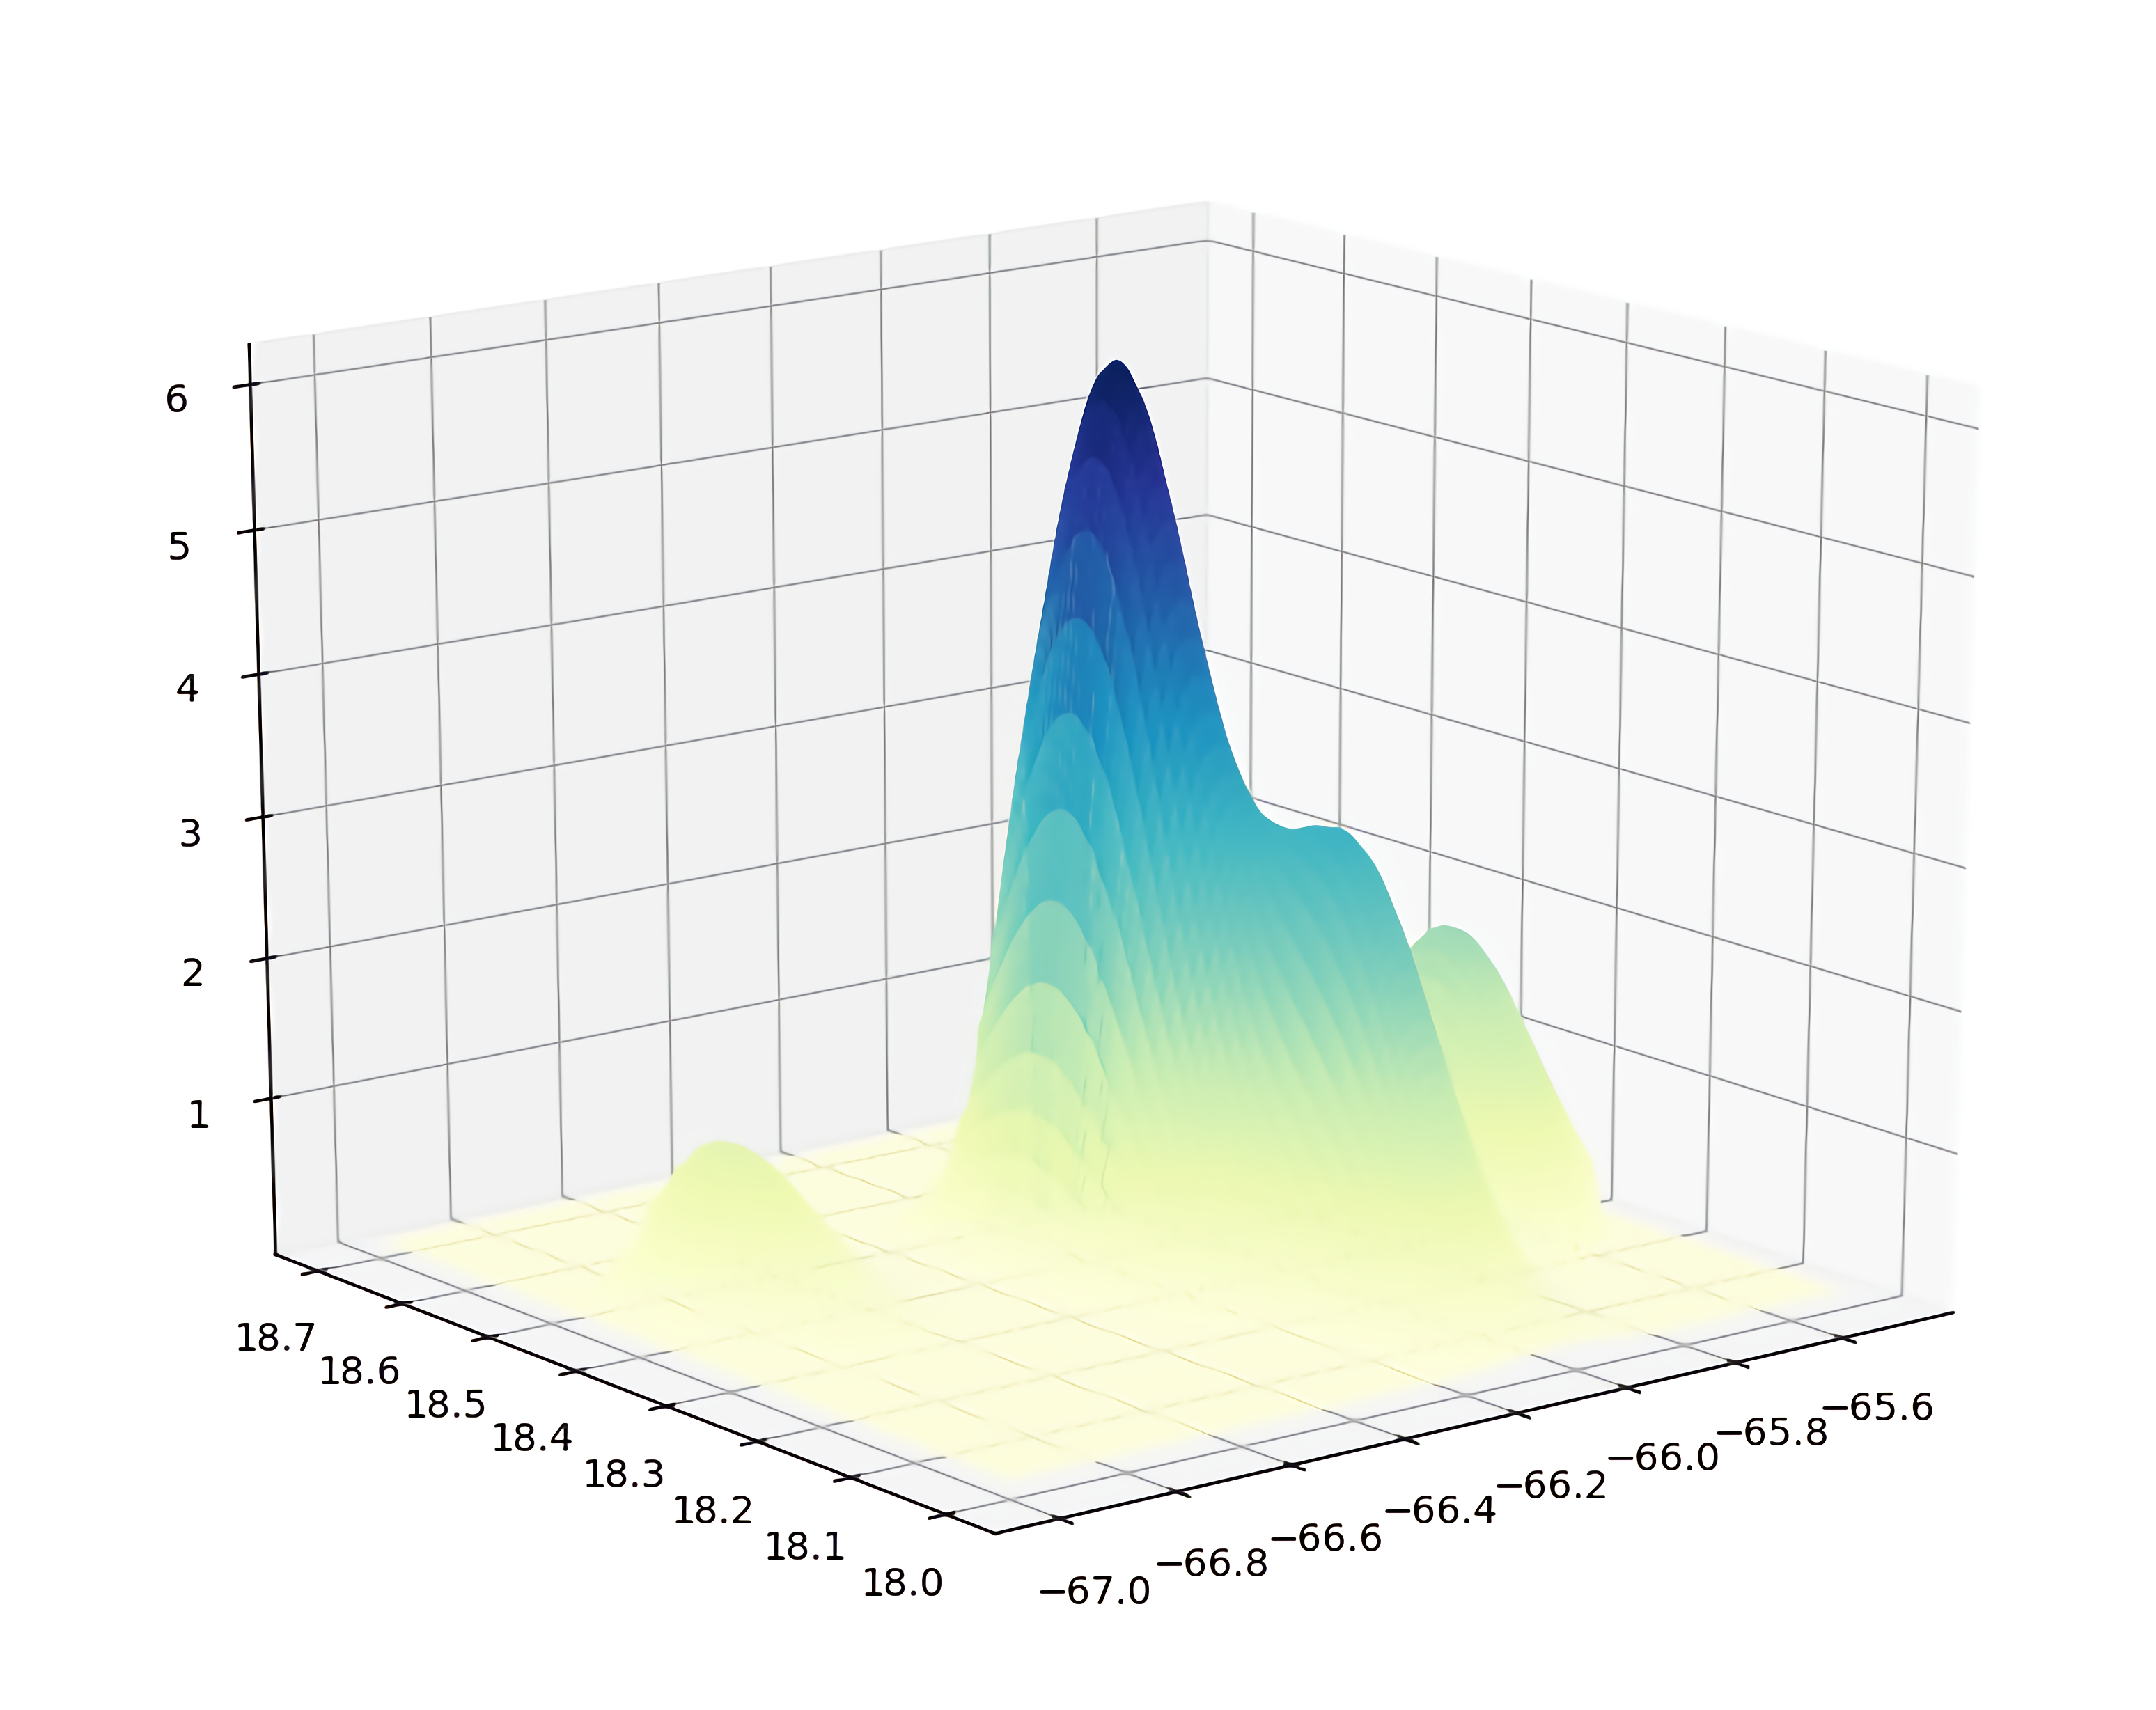
\includegraphics[height=6cm,width=10cm]{figures/importance.png}
    \caption{Importance Distribution of Medical Demand}
    \label{Fig:impo}
\end{figure}

\subsubsection{Battery Consumption}\label{Subsub:batt}

Total flight time of a single drone differs, as \emph{the weight of cargo} should be taken into account. After investigating kinds of droness for similar purposes and researching relevant factors that influence flight time, we generate an equation of drones's flight time $(t_i,i\in\{A,B,C,D,E,F,G,H\})$ in Equation \eqref{Equa:ener}~\cite{DroneFlightTime}.

\begin{equation}\label{Equa:ener}
    T_i = \frac{c_i \cdot d_i \cdot v_i}{a_i \cdot p_i}
\end{equation}

where:
\begin{itemize}
\item $T_i$ stands for the total flight time of each drone;
\item $c_i$ is the battery capacity of each drone;
\item $d_i$ is the battery discharge of each drone that is allowed for during the flight, which is typically a default value ;
\item $v_i$ is the voltage of each drone;
\item $a_i$ is the all-up weight of each drone;
\item $p_i$ is the power required to lift one kilogram of equipment.
\end{itemize}

Based on the given \emph{Flight Time No Cargo} data in $Attachment\,2$, and rated parameters of batteries, $a_i$ or \emph{net weight} of each drone can be obtained. We use the parameter $m_i$ to denote net weight of each drone. As soon as the drone is loaded with packaged cargo, $a_i$ equals to the \emph{sum} of $m_i$ and payload carried. In this way, Equation \ref{Equa:ener} turns to Equation \ref{Equa:time} as follows:

\begin{equation}\label{Equa:time}
    T_i^{'} = \frac{c_i \cdot d_i \cdot v_i \cdot T_i \cdot p_i}{c_i \cdot d_i \cdot v_i + m_i \cdot T_i \cdot p_i}
\end{equation}

In Route Selection Model, each drone only has two status, namely \emph{cargo occupied} or \emph{cargo vacant}. Therefore, there are two kinds of total flight time, which represents max delivery time possible$(T_{i1})$ and max return time possible $(T_{i2})$. $T_{i1}$ and $T_{i2}$ can be generated from Equation \eqref{Equa:ener} and Equation \eqref{Equa:time}. However, the outright battery capacity is a limited number, so there exists a restricting equation.

\begin{equation}\label{Equa:rest}
\frac{t_{i1}}{T_{i1}}+\frac{t_{i2}}{T_{i2}} = 1
\end{equation}

where:

\begin{itemize}
    \item $t_{i1}$ is the actual time spent for Delivery;
    \item $t_{i2}$ is the actual time spent for Return.
\end{itemize}

In Equation \eqref{Equa:rest}, there are only two unknown numbers, $t_{i1}$ and $t_{i2}$. After adding another equation of distance ($\frac{t_{i1}}{t_{i2}}$=$\frac{d_{i1}}{d_{i2}}$), we can calculate the values of them.


\subsubsection{Three Selected Locations}
Depending on demand distribution and battery consumption, we plot Figure \ref{Fig:circ}. In the picture, the orange circle represents the flight radius of Drone F, blue for Drone C, and green for Drone B. The radius of each circle is determined by Equation \eqref{Equa:rest}, where $t_{i1}$ equals to $t_{i2}$, and $T_{i1}$ and $T_{i2}$ are already known. The radius gives the max coverage of any circle. As is seen from the picture, there are two different sets of circles, namely one on the eastern and the western edge and the other in the middle. Accordingly, we provide two means to finalize our selection of three container locations.

\begin{figure}[htbp]
    \centering
    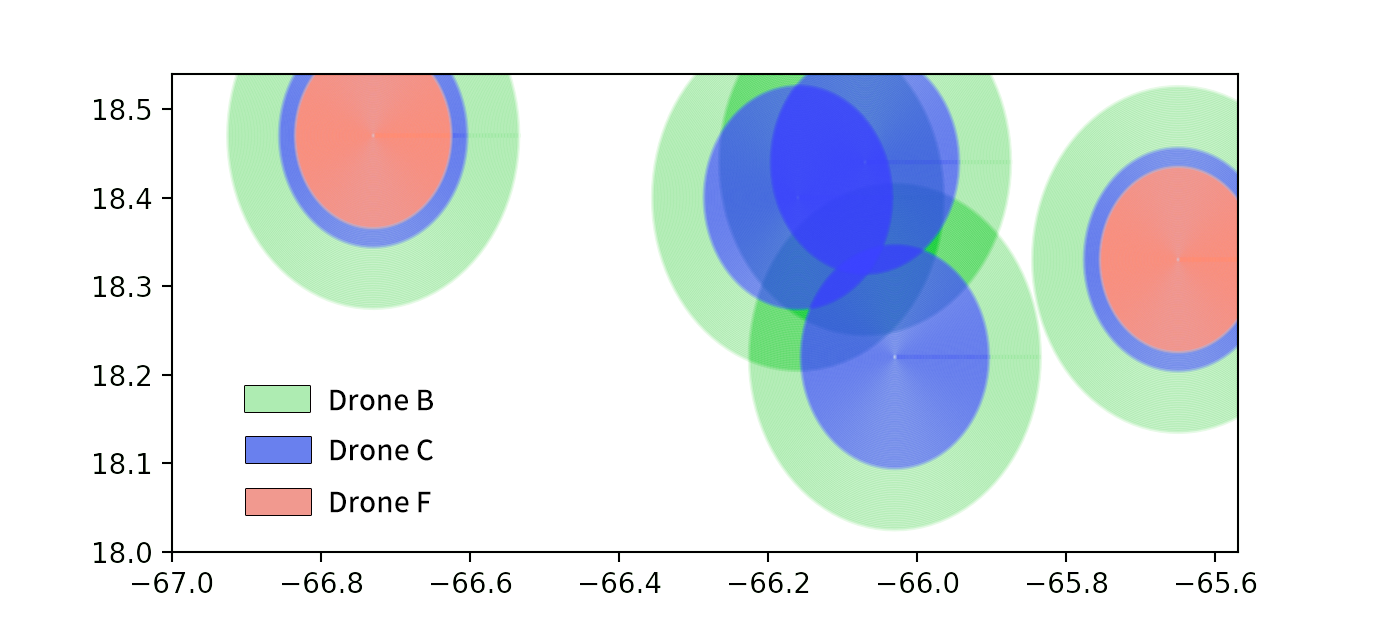
\includegraphics[width=11cm]{figures/radius4.png}
    \caption{Three Demand-Related Regions}
    \label{Fig:circ}
\end{figure}

\paragraph{Middle Region} For the region in the middle we first focus on the overlapping part of three smaller circles(or blue circles). Then, we calculate the circumferential circle center of the overlapping part, and determine it as the container location for the three hospitals in the middle. This is the place where any type of the drone deployed can reach any of the hospital in this region. Since this place have high demand for medical packages, as shown in Figure \ref{Fig:impo}, we will call this place \emph{delivery-prioritized region} in the following part.

\begin{figure}
    \centering
    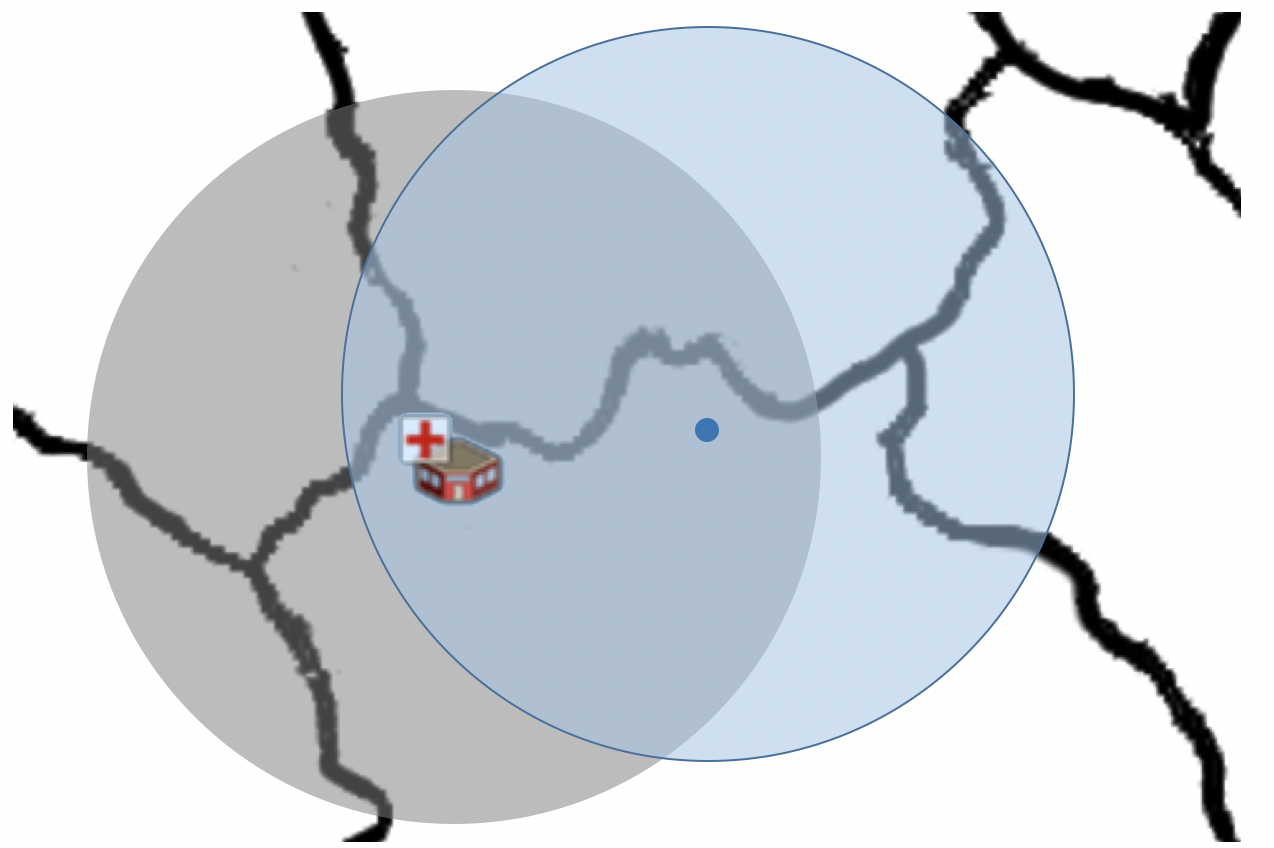
\includegraphics[width=10cm]{figures/find_location.png}
    \caption{Find Optimal Location for Containers on Side Regions}
    \label{Fig:fdlc}
\end{figure}

\paragraph{Side Regions} For both regions on the east and west, the demand for medical packages is low, thus offering us sufficient space for video reconnaissance. So in these two regions, our top priority is to maximize the road coverage. We denote the set of road points as $R$. Then we define the indicator function $I_R(x, y)$ \cite{ProbabilityTextbook}:
\begin{equation}
    I_R = \left\{
    \begin{aligned}
    &1, &(x, y)\in R \\
    &0, &(x, y)\notin R
    \end{aligned}
    \right.
    \label{Equ:indi}
\end{equation}
In these two regions, there is only one hospital, respectively. We draw a circle $C_H$ centered at the hospital with radius $r_m$. $r_m$ should be the minimum reachable radius of all the drones deployed in this region. In our model, this is the radius of Drone F. We choose a point $P_C\in C_H$ and draw another circle $C_D$ centered at $P_C$ with radius $r_s$. We estimate road area within the $i$th region by
\begin{equation}
    S_i = \iint_{C_D} I_R(x, y) \mathrm{d}x\mathrm{d}y
\end{equation}
The method is shown in Figure Here we can use \textbf{Simulated Annealing(SA)} to find $C_D$ with the largest road area. Simulated Annealing somehow resembles Metropolis-Hastings Algorithm in their "accept by probability" strategy. The difference is that SA aims to find the optimal solution while MHA aims to generate samples from a function. 

Table \ref{Tab:thre} and Figure \ref{Fig:loca} showcase specific locations for three containers respectively.

\begin{figure}[htbp]
    \centering
    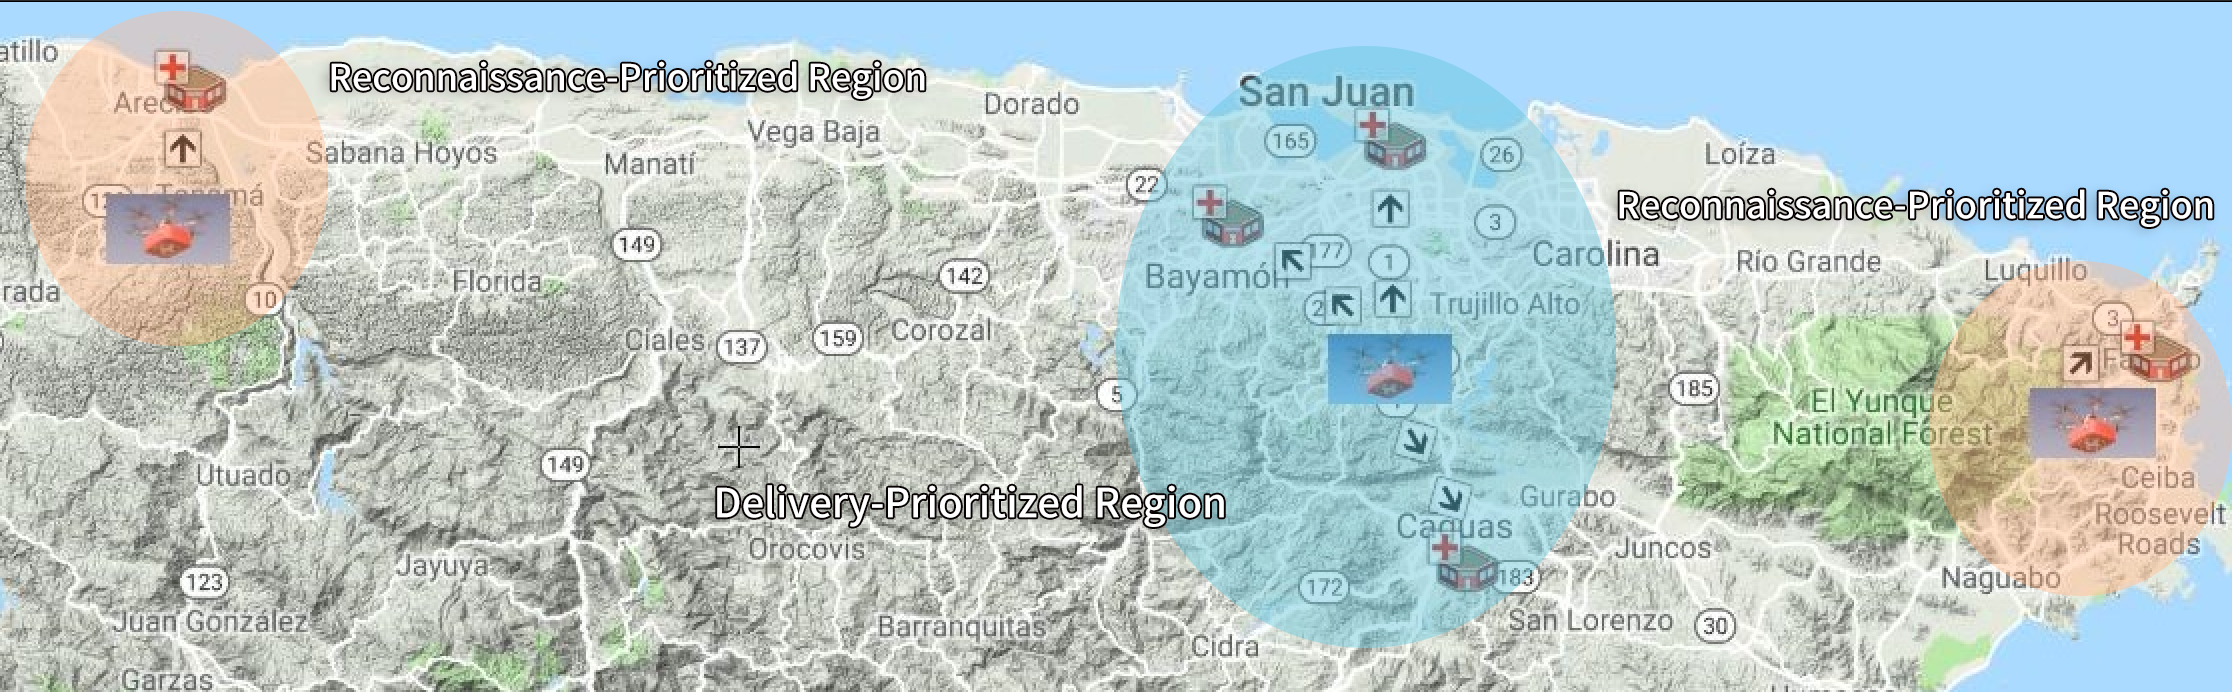
\includegraphics[width=13cm]{figures/location.jpg}
    \caption{Three Container Locations}
    \label{Fig:loca}
\end{figure}

\begin{table}[htbp]
    \centering
    \begin{tabular}{c|c c}
    \hline
    Container Location & Longitude & Latitude\\
    \hline
         1 & -65.6848 & 18.2934\\
         2 & -66.0710 & 18.3200\\
         3 & -66.7421 & 18.3932\\
    \hline
    \end{tabular}
    \caption{Three Container Locations}
    \label{Tab:thre}
\end{table}


\subsection{Route Selection Model}
As is mentioned before, the three regions are divided into two kinds, the eastern and western two regions as well as the middle region. Since the first two regions only has one hospital to serve, their mission is mainly reconnaissance-prioritized. Since there are three hospitals to serve in the middle region, the drone' mission there is mainly delivery-prioritized.

\subsubsection{Delivery-Prioritized Region}\label{Subsub:deli}
Now we shift our attention to the delivery-prioritized region, which refers to the part around San Juan. We call this place \emph{delivery-prioritized} because we have to serve three of the five hospitals in this region. In this place, the efficiency of transporting medical packages to hospitals is the top priority, while the video reconnaissance work should not be ignored. With this situation in consideration, we first propose a strategy for each drone in the container to load medical packages into its bay and transport to a certain hospital. Then the drone can decide its path of returning back, which maximizes road coverage.

When a drone is about to take off, the content of the bay tied to a drone taking off must be decided. Here we can randomly choose a packaging strategy that satisfies the payload capabilities of the drone. The packaging strategy candidates are already provided in Container Internal Placement Model. The best combination of packaging strategies for all drones can be later figured out by a heuristic algorithm.

As demonstrated in Destination Selection Model, the location of the container in delivery-prioritized region is chosen in such a way that the drone of both type deployed, i.e. Drone B and Drone C, can reach any of the hospital in delivery-prioritized region and return safely. After the bay is packaged, a drone randomly choose a hospital in this region. The best distribution of the drone flow can also be figured out by a heuristic algorithm.

After delivering the medical packages, the drone has to return to container and wait for charging. Since the drone has completed its major task, the efficiency of video reconnaissance should be considered. If the drone returns in straight line, the margin of the battery life may not be fulled exploited to assess road conditions. However, as the power is not so efficient, the returning route cannot be too twisted, in which case the drone may have difficulty reaching container. 

Here we use \textbf{Quadratic B\'{e}zier Curve} \cite{BezierCurve} to depict this returning route. B\'{e}zier Curve is widely used in many fields, such as computer graphics and robotics. The $n$th order of B\'{e}zier Curve is determined by $n+1$ points $P_0, P_1, ..., P_{n}$. A Quadratic B\'{e}zier Curve can be expressed mathematically as:
\begin{equation}
    \mathbf{B}(t)=(1-t)^2\mathbf{P}_0 + 2t(1-t)\mathbf{P}_1 + t^2\mathbf{P}_2, 0 \leq t \leq 1
    \label{Equ:bezr}
\end{equation}

\begin{figure}[htbp]
    \centering
    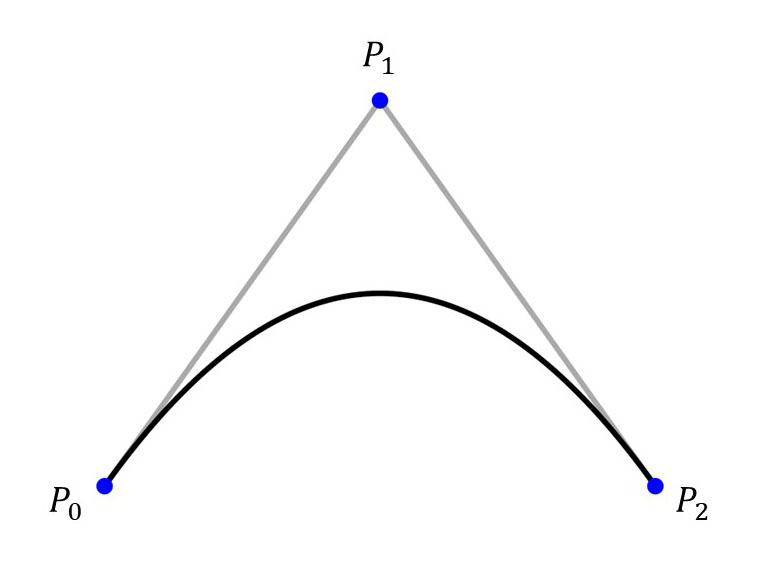
\includegraphics[width=8cm,height=5cm]{figures/bezier.jpg}
    \caption{Plot of Quadratic B\'{e}zier Curve}
    \label{Fig:bezr}
\end{figure}

A plot of Quadratic B\'{e}zier Curve is shown in Figure \ref{Fig:bezr}. Higher orders of B\'{e}zier Curve are also available, but need more control points and may look more twisted. That's why we choose the quadratic one. 

The length of a B\'{e}zier Curve can be expressed by the following integral:
\begin{equation}
\begin{aligned}
    |\mathbf{B}| &= \int_B \mathrm{d}l = \int_0^1 \sqrt{[P_x'(t)]^2 + [P_y'(t)]^2} \mathrm{d}t \\
    &= \int_0^1 2\sqrt{[-(1-t)P_{0x}+(1-2t)P_{1x}+tP_{2x}]^2 + [-(1-t)P_{0y}+(1-2t)P_{1y}+tP_{2y}]^2} \mathrm{d}t
\end{aligned}
\label{Equ:bezl}
\end{equation}
Note that this equation is rather difficult to get its analytic solution. In practice, we subdivide this curve into several line segments and compute the sum of their lengths. With Equation \eqref{Equ:bezl}, we can get the length of a drone's returning route.

A drone has to assess road conditions in Puerto Rico, so a criterion must be defined to evaluate the effectiveness of video capture. First we consider a certain point on the route. Suppose a drone with field of view \cite{FieldOfView} $f$ is at height $h_D$, then the ground area covered by the camera can be approximated by a circle of radius $r_c = h_D \cdot f/2$. With this in mind, we can define road coverage of a route $\mathbf{B}$ as:
\begin{equation}
    CV(\mathbf{B}) = \frac{w_r}{\pi r_c^2} \int_B\mathrm{d}l \iint_{C_t} I_R(x, y) \mathrm{d}x\mathrm{d}y
    \label{Equ:rtcv}
\end{equation}
where:
\begin{itemize}
    \item $w_r$ is the average width of road
    \item $C_t$ is the circle area centered at $\mathbf{B}$(t) with radius $r_f$
    \item $I_{R}(x, y)$ is the indicator function which indicates whether the point $(x, y)$ is on roads.
\end{itemize}

\begin{figure}[ht]
	\centering
	\begin{minipage}[t]{0.48\textwidth}
		\centering
		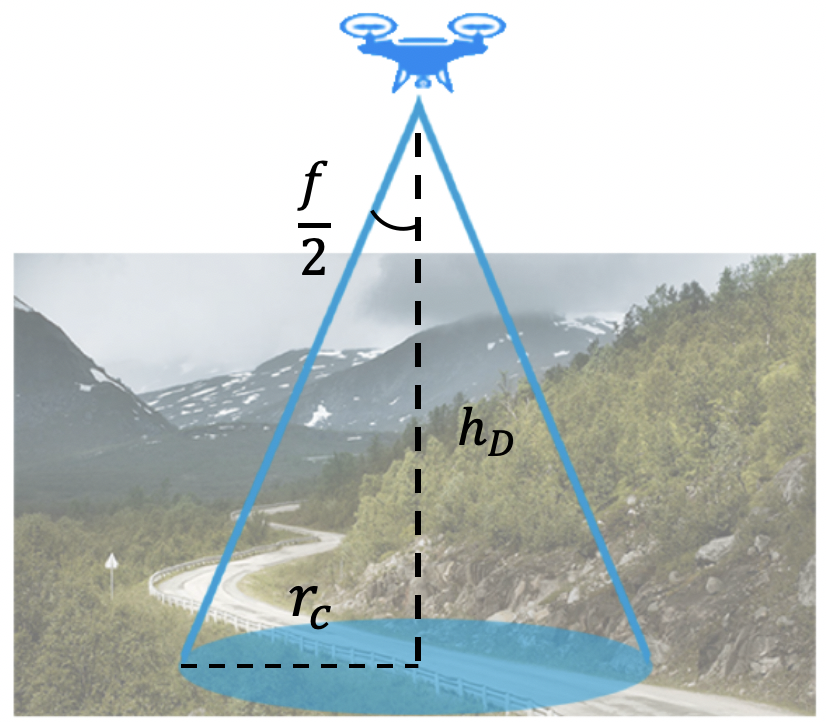
\includegraphics[width=8cm,height=7cm]{figures/fov.png}
		\centering{(a) Road Coverage on a Single Point}
	\end{minipage}
	\begin{minipage}[t]{0.48\textwidth}
		\centering
		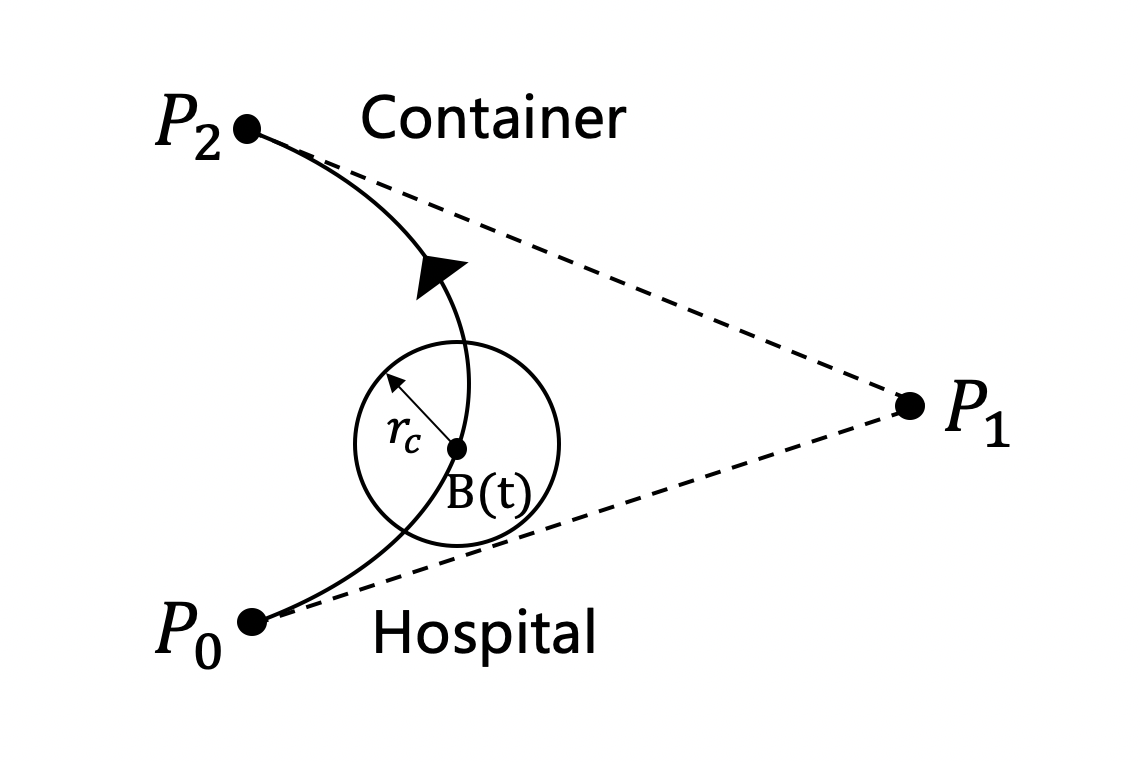
\includegraphics[width=8cm]{figures/route_coverage.png}
        \centering{(b) Road Coverage along a Returning Route}
	\end{minipage}
	\caption{Determination of Road Coverage}
	\label{Fig:rdcv}
\end{figure}

After defining the coverage $CV(\mathbf{B})$, we have to find a way that can maximize road coverage on the returning route. Because of the difficulty of integrating over the whole curve, we resort to a local search method. We connect the hospital and container with a straight line segment $l_s$. Then we draw a line segment $l_p$ of length $2|l_s|$ which is perpendicular to $l_s$ and its midpoint coincides with the one of $l_s$. We divide $l_p$ into several segments, put B\'{e}zier Curve control point $P_1$ at each endpoint of these segments and try to find the position which has the largest $CV(\mathbf{B})$. The method is demonstrated in Figure \ref{Fig:lcsr}.

\begin{figure}[htbp]
    \centering
    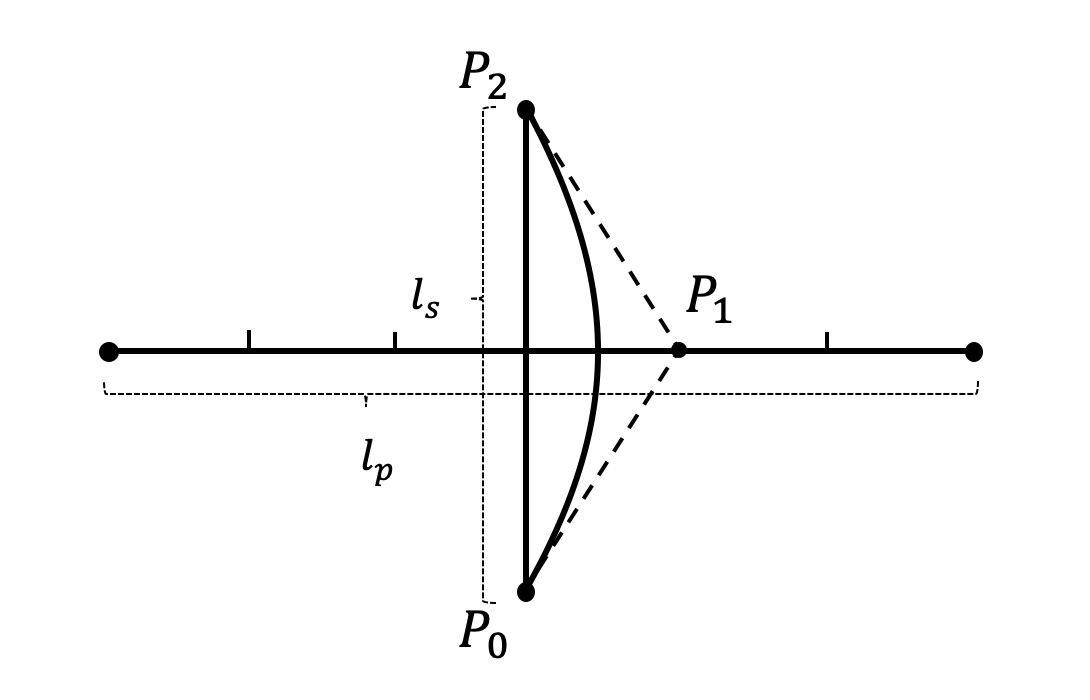
\includegraphics[width=10cm]{figures/local_search_route.png}
    \caption{Local Search of Best-Covering Route}
    \label{Fig:lcsr}
\end{figure}

\subsubsection{Reconnaissance-Prioritized Region}\label{Subsub:reco}
In this part we discuss the other two regions: the one on the north-east coast and the one on the north-west cost. The two share in common that there is only one hospital in each of the region and the demand for medical packages are relatively low. In this region, the delivery is not so important as it is in delivery-prioritized one. More drones should be deployed to assess the road conditions instead of sending goods. The deployment strategy could be quite different from the one discussed in delivery-prioritized region.

Since the demand for goods is low, a small number of drones sending a fixed set of medical packages can sufficiently meet the demand. Therefore, no randomness is involved in this region and we don't need any heuristic algorithm to find an optimal solution. Among all the drones in the containers transported to these two locations, Drone F is only capable of delivering goods, so the two Drone F's should shoulder the responsibility of transporting medical packages. The bay packaging for Drone F's in these regions can specified explicitly, according to the demand of target hospitals. The other two types, Drone B and Drone C are assigned to assess nearby road conditions. 

For video reconnaissance-oriented drones, the routes design should be different from the one discussed in previous part, in that it doesn't have to transport packages and should fully explore the roads nearby. The strategy is that when a drone takes off, it searches for the nearest road that has not been discovered and march to that point. It follows the roads and captures videos of them, while keeping track of the distance from the container and judging whether it should return, in case it may not be able to get back if battery life runs out. If the battery life could not support drone to cruise further, it returns to the container along the straight line route.

The situation gets complicated if we consider of the variable shapes of roads. In that way, the total road coverage of drones may be hard to expect. Here we firstly consider a simplified case, as shown in Figure \ref{Fig:vdsr} . Suppose there is a semi-infinite road. A container is away from the road by $d$. Drones are released from containers, one by one. The route of the first, second and third drone are marked on the figure. The furthest point on axis X on the road the $i$th drone can reach is denoted as $x_i$, and the length of road covered by the $i$th drone $l_i$. Therefore, we have $l_i=x_i-x_{i-1}$. Suppose the maximum length a drone can fly through is $s$, using Pythagorean theorem, we have:
\begin{equation}
    \sqrt{d^2+x_{i-1}^2} + l_i + \sqrt{d^2+x_i^2} = s
    \label{Equ:drvr}
\end{equation}
According to Equation \eqref{Equ:drvr}, we can get the recursion formula of series $x_i$:
\begin{equation}
    \left\{
    \begin{aligned}
    &x_0 = 0 \\
    &x_i = \frac{(s + x_{i-1} - \sqrt{d^2 + x_{i-1}^2})^2 - d^2}{2(s + x_{i-1} - \sqrt{d^2 + x_{i-1}^2})}
    \end{aligned}
    \right.
\end{equation}

\begin{figure}[htbp]
    \centering
    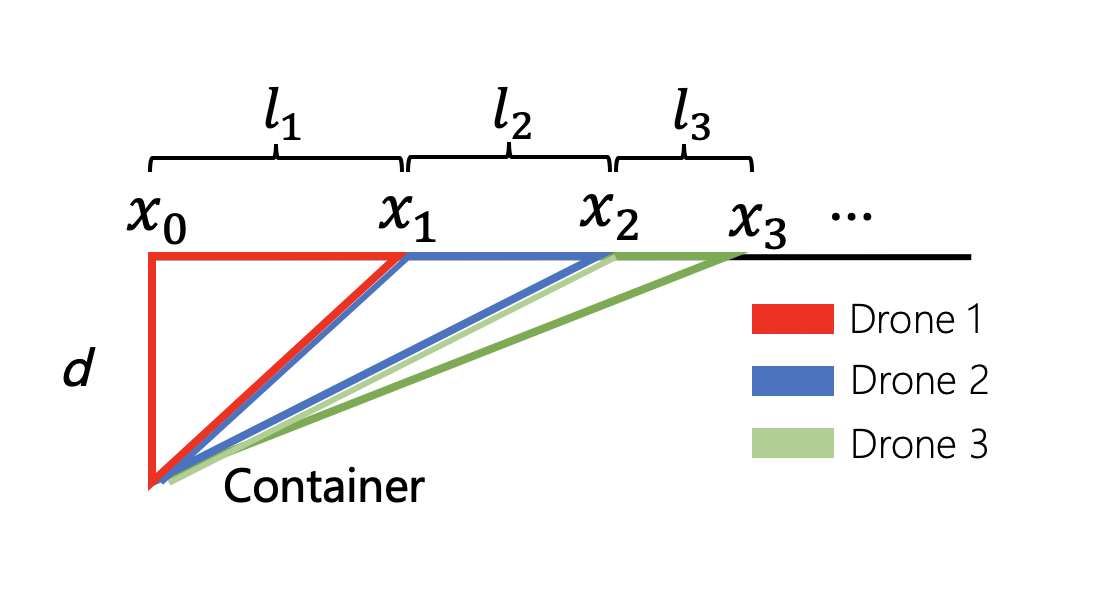
\includegraphics[width=10cm]{figures/video_drone_path.png}
    \caption{A Simplified Case of Drone Routes for Video Reconnaissance}
    \label{Fig:vdsr}
\end{figure}

We set $s$ to be the average flight distance of drones in the fleet, and $d$ to be average distance from the containers to the roads nearby. We compute the first several elements in the series and plot it on the graph. We find that this series can be fitted with an exponential function. See Figure \ref{Fig:cvft} for the plotted graph. We find that the the more drones we put into use, the less coverage a single drone can produce. That's because when more drones are launched, the farther the drone has to fly to reach the starting location of video capture. Since the battery life of a drone is fixed, the distance that a drone can actually spend on road assessment decreases continuously. 

The actual road condition may be far more complicated than the one discussed preciously, but we can infer that they have similar growing trend. So we can define the coverage function of the $i$th reconnaissance-prioritized region $CV_i$ as the following:
\begin{equation}\label{Equ:cs}
    CV_i = S_i(1 - e^{-\alpha N_{D,i}})
\end{equation}
where 
\begin{itemize}
    \item $S_i$ is the road area that is reachable by drones with straight line routes in the $i$th reconnaissance-prioritized region. 
    \item $N_{D,i}$ is the number of drones assigned to carry out video reconnaissance work 
\end{itemize}
In our implementation, we set $\alpha$ to be 1.7293. The sensitivity analysis of this parameter is discussed in Section \ref{Sec:mode}.

\begin{figure}[htbp]
    \centering
    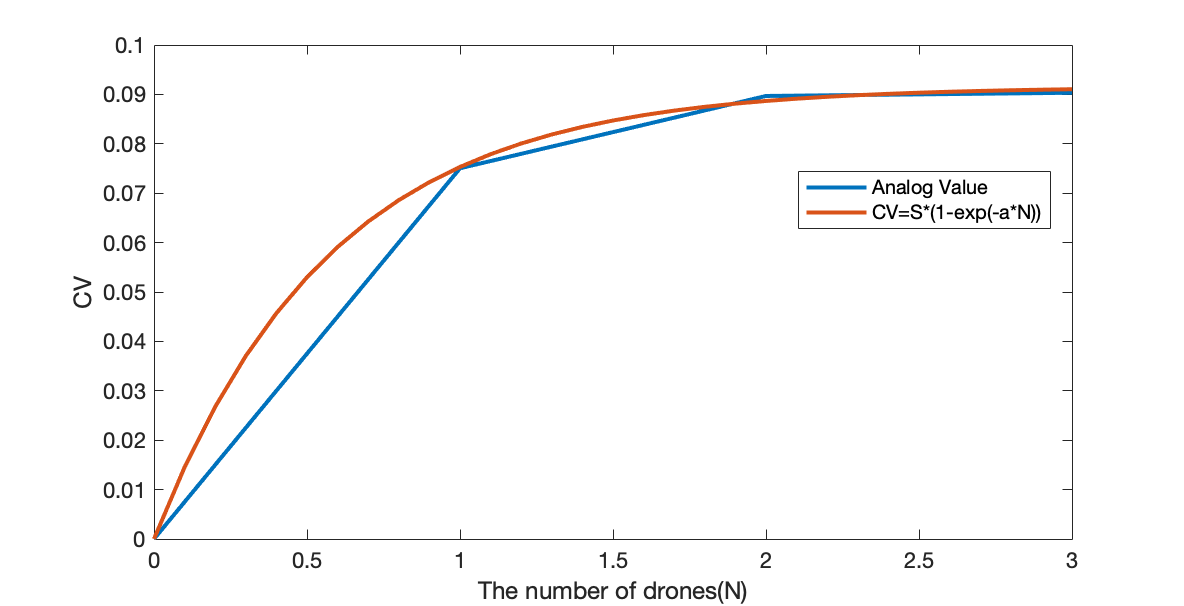
\includegraphics[width=12cm,height=6cm]{figures/alpha7.png}
    \caption{Plot of the Series and Fitting Function}
    \label{Fig:cvft}
\end{figure}

\subsubsection{Route Evaluation}
We have already discussed the situation in delivery-prioritized and reconnaissance-prioritized regions. To eventually find the combination of bay packaging and drone dispatch strategy that maximizes the general efficiency of delivering response system to Puerto Rico, including both package delivery and video reconnaissance, we have to firstly define an evaluation function that assesses the comprehensive performance. 

For the package delivery part, each hospital has its certain demand for medical packages, and each container has drones that are different in their payload. The problem may seem complicated if we want to take all of the supply and demand into consideration. Here we follow the Cask Principle, which claims that the performance of a system is determined by its weakest part. In the case of package delivery, this refers to the minimum number of days any hospital can sustain itself without additional packages. This seems reasonable in the case of package delivery, because whenever any of the hospital is in lack of the any type of the package, the company has to deliver packages again. We want a delivery that can support all the hospitals on the island to survive more days. Suppose package demand of the $t$th type package in the $s$the hospital is recorded in $n_{s,t}$, and the actual delivered package of the $t$th type to the $s$th hospital is $n'_{s,t}$, the sustaining days for the $t$th package in the $s$th hospital is:
\begin{equation}
    m_{s,t} = \left\{
    \begin{aligned}
    &\biggl\lfloor\frac{n'_{s,t}}{n_{s,t}}\biggr\rfloor, &n_{s,t}\neq 0 \\
    &\infty, &n_{s,t}=0
    \end{aligned}
    \right.
\end{equation}
Then the day interval between two deliveries $m_d$ can be expressed as:
\begin{equation}
    m_d = \min\limits_{1\leq i\leq 5, 1\leq j\leq 3}\{n_{s,t}\}
\end{equation}

Then we can define the delivery term $E_d$:
\begin{equation}
    E_d = \frac{2}{1+e^{-km_d}}-1
    \label{Equ:dlev}
\end{equation}
This function looks similar to Logistic function \cite{LogisticFunction}. The difference is that this function maps natural numbers $\mathbb{N}$ to real numbers in $[0,1)$. When $m_d$ decreases to numbers around zero, the value of this function falls dramatically. This property helps avoid extremely low $m_d$ and ensures the effectiveness of delivery. 

As for the video reconnaissance evaluation, we just need to compute the ratio of the sum of the road area covered in all regions $CV_i$ to the total road area $S_{all}$:
\begin{equation}
    E_v = \frac{\sum_{i=1}^3 CV_i}{S_{all}}
    \label{Equ:vrev}
\end{equation}

Then we define our final evaluation function $E$:
\begin{equation}
    E = E_d + E_v = \frac{2}{1+e^{-km_d}} - 1 + \frac{\sum_{i=1}^3 CV_i}{S_{all}}
\end{equation}

With this equation, \textbf{Simulated Annealing} can be used to find the optimal solution. Just before we run SA, the last thing that should be clarified is the randomness involved in the process, and the dimension of the problem. For the reconnaissance-prioritized region, the container packaging strategy and drone routes are already determined, so there is no randomness in this part. For the delivery-prioritized region, we use local search to determine returning routes, so there is also no randomness. However, we randomly choose the bay packaging strategy and the hospital to deliver for each drone. Therefore, the maximum dimension of this problem is twice the number of the drones deployed in the delivery-prioritized region. If we reuse samples in our implementation, the dimension may be reduced.




\subsubsection{Realistic Operation}\label{Subsub:real}

\paragraph{Bay Packing}In Section \ref{Subsub:cont}, we generate two kinds of drone fleets for container configurations. After generating the optimal outcomes, we employ Drone Fleet I for two reconnaissance-prioritized regions in the side, and Drone Fleet II for one delivery-prioritized region on both sides. We provide cargo bay configurations for each container in Table \ref{Tab:seto1} and Table \ref{Tab:seto2}.

\begin{table}[htbp]
  \centering
  \caption{Set of Packages for Drone Fleet II}
    \begin{tabular}{ccccc}
    \hline
    Container & MED 1 & MED 2 & MED 3 & Quantity \\
    \hline
    1     & 3     & 0     & 3     & 2 \\
    3     & 6     & 0     & 1     & 2 \\
    \hline
    \end{tabular}%
  \label{Tab:seto1}%
\end{table}%

\begin{table}[htbp]
  \centering
  \caption{Set of Packages for Drone Fleet I}
    \begin{tabular}{ccccccccc}
    \hline
    \multicolumn{4}{c}{Drone Fleet I Bay 1(Drone B)} &       & \multicolumn{4}{c}{Drone Fleet I Bay (Drone C)} \\
    MED 1 & MED 2 & MED 3 & Quantity &       & MED 1 & MED 2 & MED 3 & Quantity \\
    \hline
    1     & 1     & 0     & 7     &       & 4     & 1     & 1     & 2 \\
    0     & 2     & 1     & 5     &       & 2     & 2     & 2     & 1 \\
    1     & 0     & 1     & 4     &       & 1     & 1     & 3     & 1 \\
    0     & 0     & 2     & 4     &       & 1     & 0     & 4     & 1 \\
    2     & 0     & 0     & 3     &       & 2     & 0     & 3     & 1 \\
    0     & 0     & 2     & 2     &       & 5     & 0     & 1     & 1 \\
    0     & 4     & 0     & 2     &       & 3     & 1     & 2     & 1 \\
    1     & 2     & 0     & 2     &       & 4     & 0     & 2     & 1 \\
    \hline
    5(sum) & 9(sum) & 6(sum) & 29(sum) &  & 22(sum)    & 5(sum)     & 18(sum)    & 9(sum)\\
    \hline
    \end{tabular}%
  \label{Tab:seto2}%
\end{table}%

\noindent Afterwards, based on each drone fleet and its set of packages, we obtain satisfied demands for once flight for every hospital. Accordingly, we calculate the time interval it takes for the next flight to depart. Both are shown in Table \ref{Tab:sati}.
\begin{table}[htbp]
  \centering
  \caption{Satisfied Demands for Five Hospital and Satisfied Days}
    \begin{tabular}{c|ccc|c}
    \hline
    Hospital & MED 1 & MED 2 & MED 3 & Satisfied Days \\
    \hline
    1     & 6     & 0     & 6     & 6 \\
    2     & 18    & 6     & 8     & 8 \\
    3     & 14    & 9     & 17    & 9 \\
    4     & 13    & 10    & 15    & 6.5 \\
    5     & 12    & 0     & 2     & 12 \\
    \hline
    \end{tabular}%
  \label{Tab:sati}%
\end{table}%

\paragraph{Schedule} Since we need to ensure local hospitals' demands, and the three regions do not affect each other. Therefore, the schedule for the eastern and middle region is six days per flight, and twelve days each flight for the western region.

\noindent The whole blueprint of our operation is depicted in Figure \ref{Fig:beau}.

\paragraph{Drone Flight Plan} In the eastern and western two regions, Drone Bs and Drone Cs are completely used for video reconnaissance, they go out to reach their longest possible radius, while their definite routes are determined by Section \ref{Subsub:reco} to achieve the largest road coverage. Drone F's are only used for video reconnaissance mission when they come back, again using formulas in Section \ref{Subsub:reco} to achieve the biggest detection zone.

\noindent In the middle region, Drone Bs and Drone Cs only assess major highway conditions and roads when they return to the base. These drones choose a route to maximize road coverage, based on theory in Section \ref{Subsub:deli}.
\begin{figure}[htbp]
    \centering
    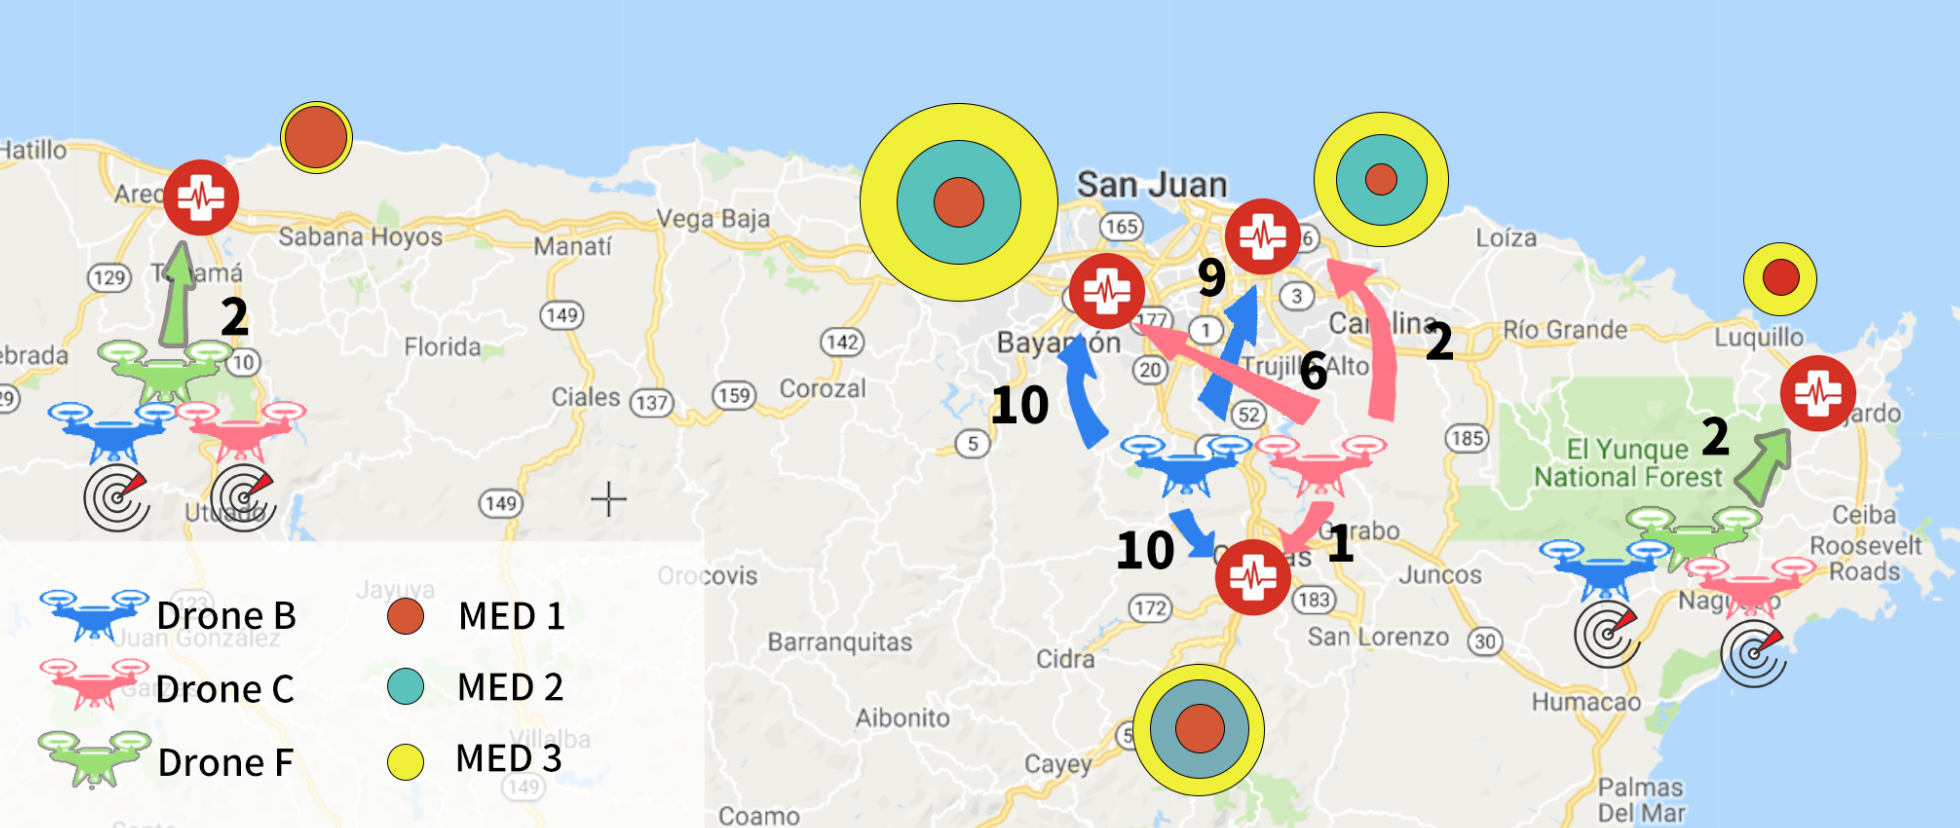
\includegraphics[width=14cm]{figures/beautiful.png}
    \caption{A Panarama of Realistic Operation}
    \label{Fig:beau}
\end{figure}

\noindent We draw a map of the highways and roads that are assessed by our drone fleets, which account for 11.596\% of the total length of highways and roads. In Figure \ref{Fig:road}, the orange roads indicate the roads already assessed by our drone fleets while the black roads are left unassessed.

\begin{figure}[htbp]
    \centering
    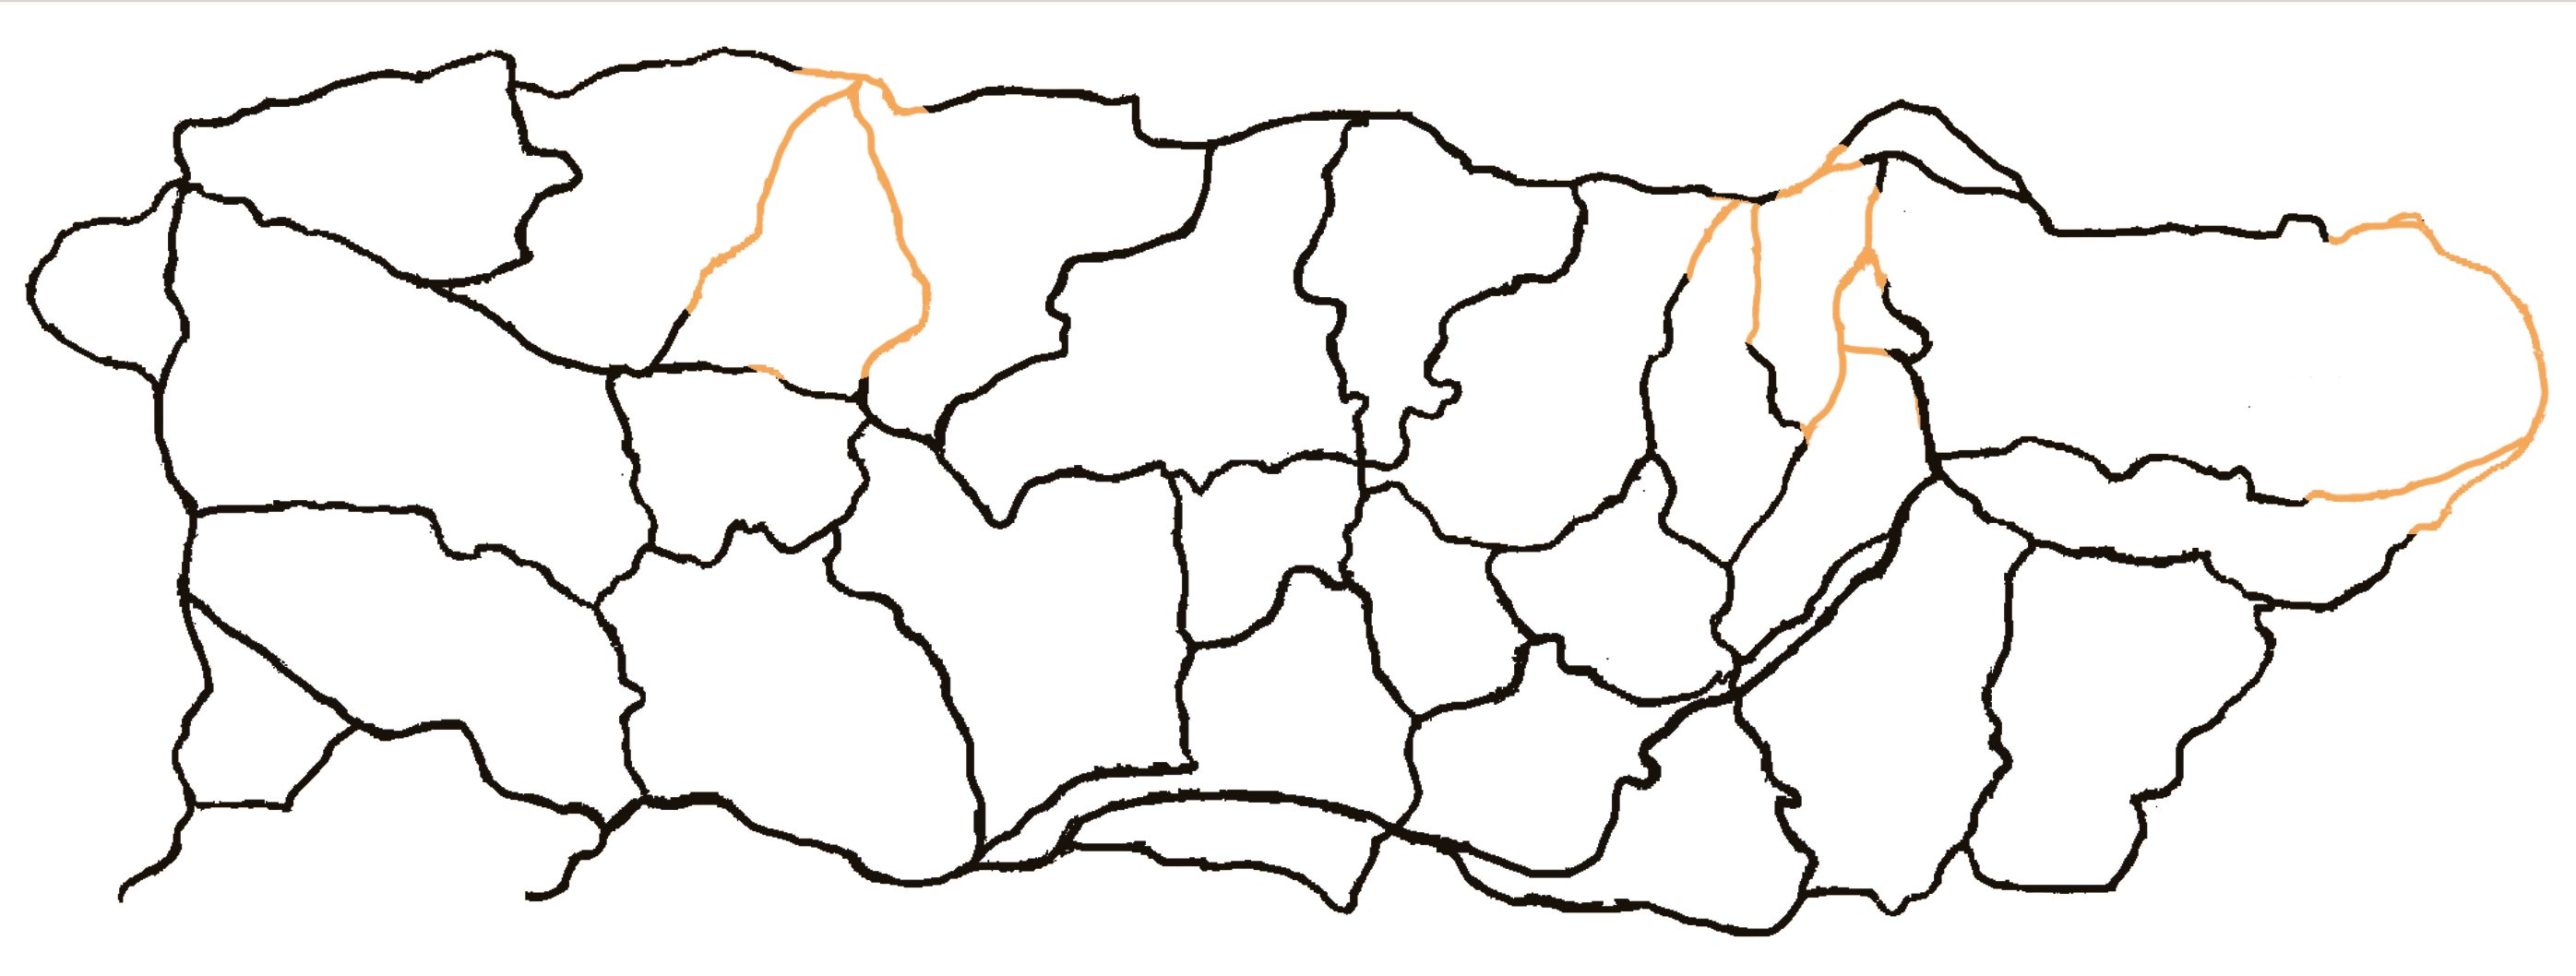
\includegraphics[width=14cm]{figures/coverage.png}
    \caption{Road Covered VS The Entire Roads}
    \label{Fig:road}
\end{figure}


\section{Model Analysis}\label{Sec:mode}

\subsection{Sensitivity Analysis}

Our model contains several parameters. We determine some of the parameters through AHP, digital image processing, and some of them by knowledge in the article or other methods. In the following subsections, we would like to produce a sensitivity analysis to show whether our model is sensitive to different values of parameters.

We will study the impact of two parameters in our model.

\subsubsection{The Impact of $\alpha$ in Drone Coverage}
\begin{figure}[htbp]
    \centering
    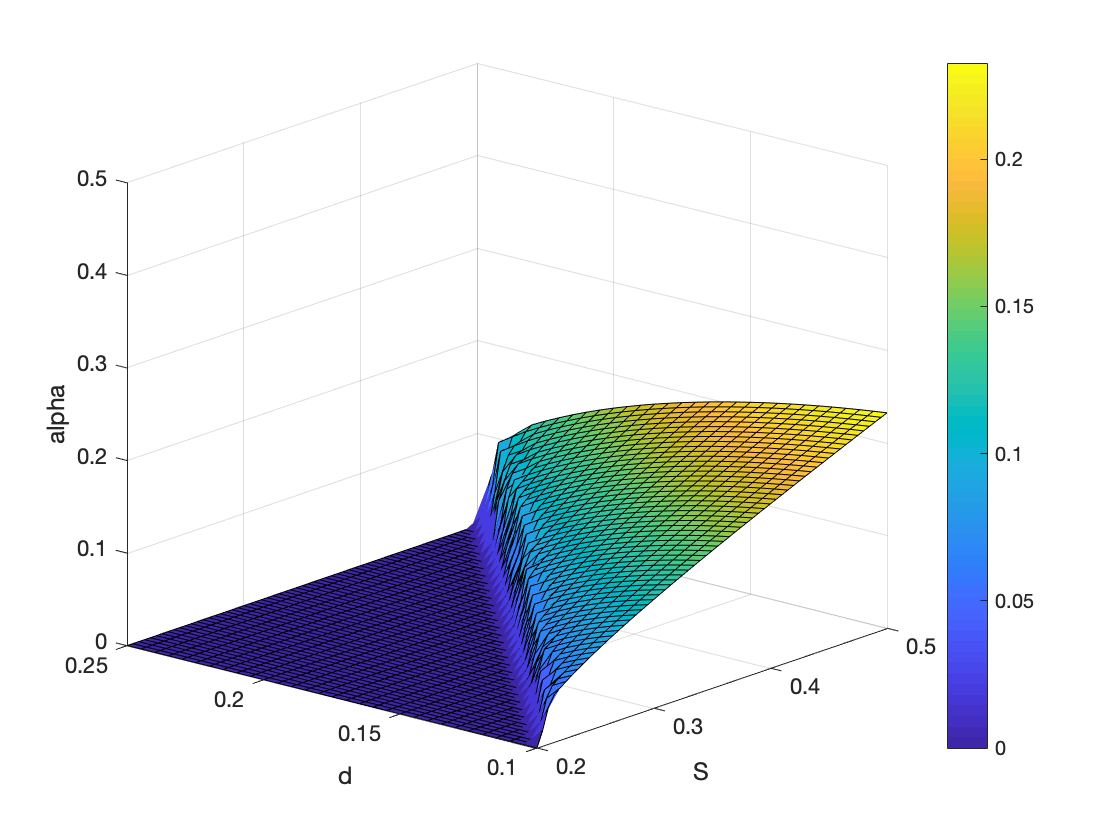
\includegraphics[width=10cm,height=6cm]{figures/alpha.png}
    \caption{Different $\alpha$ about $s$ and $d$}
    \label{fig:alpha}
\end{figure}

The parameter $\alpha$ in Equation \eqref{Equ:cs} is a result of function-fitting with given $s$ and $d$ in the simplified case of road coverage. As shown in Figure \ref{fig:alpha}, if $s$ is fixed, $\alpha$ changes a little bit with $d$. So with different $S_i$ and $N_{D,i}$, we think changing $\alpha$ in the equation does not affect the result much.

\subsubsection{The Impact of $k$ in Delivery Evaluation Function}
\begin{figure}[htbp]
    \centering
    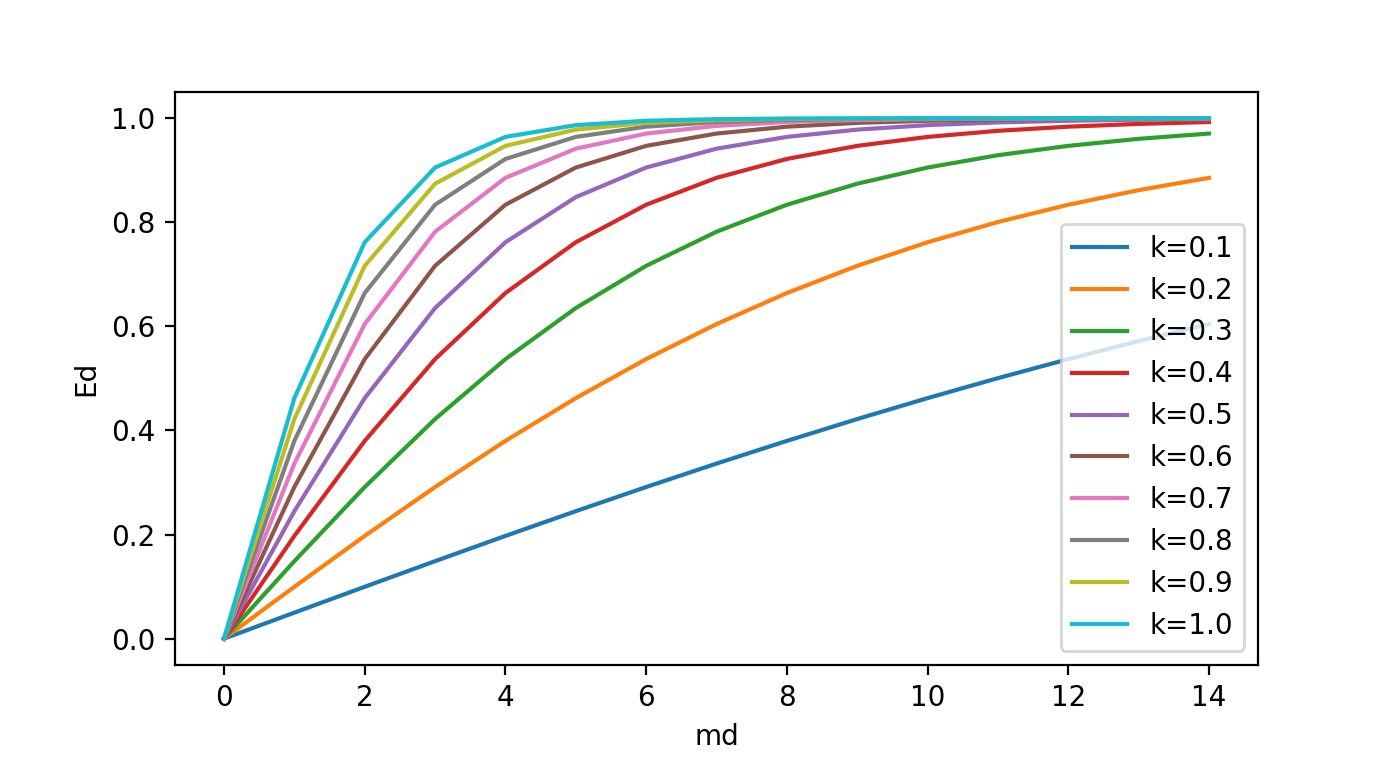
\includegraphics[width=11cm]{figures/kvalues.png}
    \caption{Different values about $k$}
    \label{fig:kvalues}
\end{figure}

The parameter $k$ in Equation \eqref{Equ:dlev} is decided by the implementor of the system. For different $k\in [0,1)$, its value will influence Equation . When $k<0.4$, it is quite hard to have high $E_d$ value, even with rather high $m_d$. $k$ can be understood as the tolerance of low $m_d$ values.


\subsection{Strengths and Weaknesses}

\subsubsection{Strengths}

\begin{enumerate}
    \item Our model is logically rigorous. Our model completely puts forward specific drone fleets ,container and bay packing solutions to HELP, Inc.
    \item We adopt interdisciplinary methods in our model. The knowledge and techniques of digital image processing are used in route selection part. 
    \item Our model is highly practial. All the theories in our model are concretely implemented and we offer comprehensive analysis and discussion of results.
    \item We make great efforts in designing our memo, to make sure the CEO of HELP, Inc. can quickly understand our solutions and therefore share it with her Board of Directors.
    \item We use fancy visualization and clear diagram to state our model.
\end{enumerate}

\subsubsection{Weaknesses}

\begin{enumerate}
    \item Simulated annealing has randomness. Because of the high dimensional constraints, we used SA as our simulation algorithm. We cannot always get the optimal outcomes for limited times of simulation.
    \item Some real-time situations are ignored. For each drone, speed cannot always be the same value, and conditions of terrain had better be considered.
    \item Although our 3D packaging algorithm considers triple rotations, we consider level rotation. It takes to much time to run the codes of triple rotations.
\end{enumerate}



\section{Conclusions}\label{Sec:conc}

Our paper provides a solution for HELP, Inc. to improve its response capabilities. We offers detailed packing configurations for drone and each of three containers. Three locations are selected in our model to position three containers respectively. We also give the routes of drone fleets, which keeps a balance between delivery mission and reconnaissance mission.

We use given data and real data online to implement our model.Since this is a high dimension problem, we implement SA to find a global optimal outcome.

Modeling outcomes are fully discussed to offer a specific memo to the CEO of HELP,Inc. We believe the anticipated medical supply demands during a potential similar future disaster scenario like Hurricane Maria will be satisfied by applying our modeling outcomes to the DroneGo disaster response system.


\section{Memo}\label{Sec:memo}
Our memo to the CEO of HELP, Inc. is shown in following two pages.
\newpage\label{page}
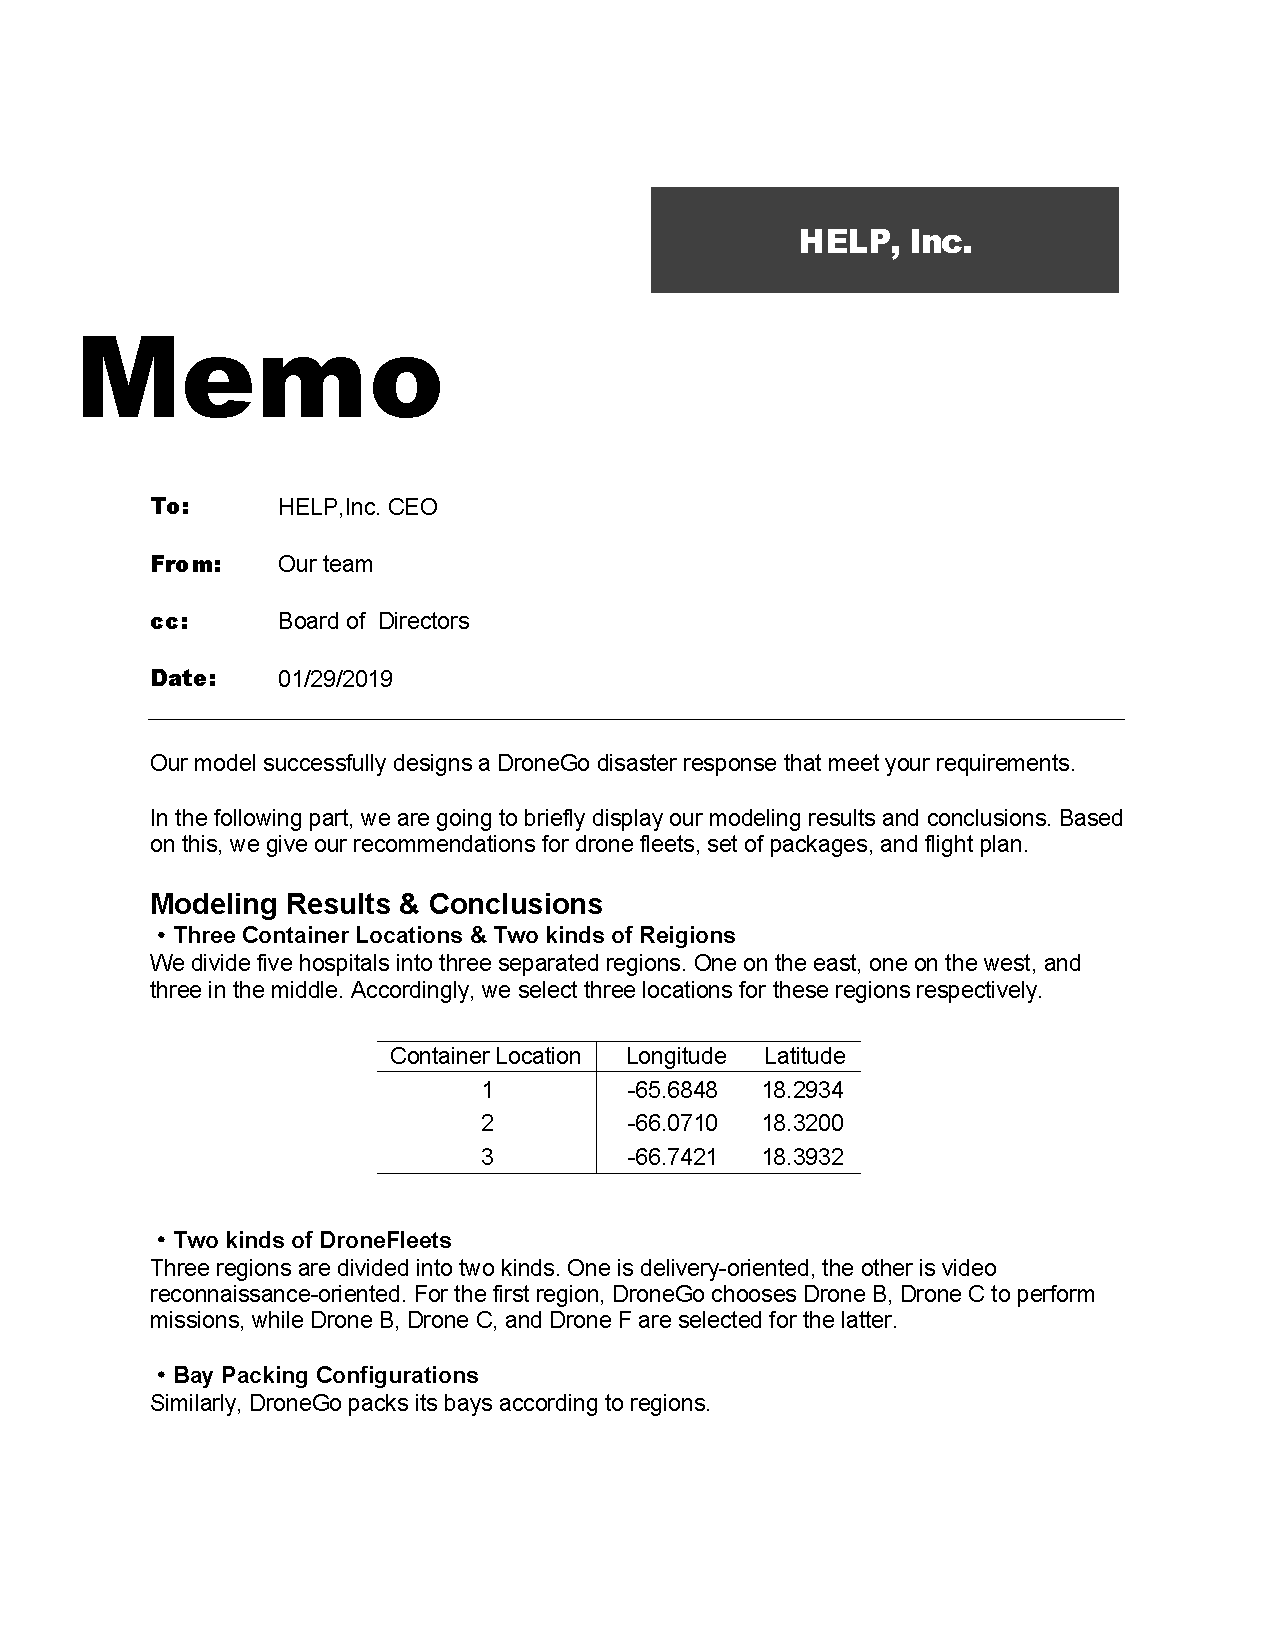
\includepdf[pages={1,2}]{HELP.pdf}




\bibliographystyle{IEEEtran}
\bibliography{newrefs}

\newpage

\begin{appendices}

\section{Alternative Configurations for Bay Packing}\label{App:alte}


\begin{table}[htbp]
  \centering
  \caption{Bay Type 1 Alternative Configurations}
    \begin{tabular}{c|c|c|c|c|c}
\hline
    \multicolumn{1}{l}{Bay} & \multicolumn{1}{l}{Med1} & \multicolumn{1}{l}{Med2} & \multicolumn{1}{l}{Med3} & \multicolumn{1}{l}{Weight} & \multicolumn{1}{l}{Utilization Rate} \\
\hline
    1     & 0     & 0     & 2     & 6     & 0.60 \\
    1     & 1     & 1     & 0     & 4     & 0.62 \\
    1     & 0     & 2     & 1     & 7     & 0.66 \\
    1     & 0     & 4     & 0     & 8     & 0.71 \\
    1     & 1     & 0     & 1     & 5     & 0.74 \\
    1     & 1     & 2     & 0     & 6     & 0.79 \\
    1     & 2     & 0     & 0     & 4     & 0.88 \\
\hline
    \end{tabular}%
\end{table}%

\begin{table}[htbp]
  \centering
  \caption{Bay Type 2 Alternative Configurations}
    \begin{tabular}{c|c|c|c|c|c}
\hline
    \multicolumn{1}{l}{Bay} & \multicolumn{1}{l}{Med1} & \multicolumn{1}{l}{Med2} & \multicolumn{1}{l}{Med3} & \multicolumn{1}{l}{Weight} & \multicolumn{1}{l}{Utilization Rate} \\
\hline
    2     & 0     & 5     & 1     & 13    & 0.14  \\
    2     & 0     & 2     & 3     & 13    & 0.15  \\
    2     & 1     & 4     & 1     & 13    & 0.17  \\
    2     & 1     & 1     & 3     & 13    & 0.18  \\
    2     & 2     & 3     & 1     & 13    & 0.20  \\
    2     & 2     & 0     & 3     & 13    & 0.21  \\
    2     & 3     & 2     & 1     & 13    & 0.23  \\
    2     & 4     & 1     & 1     & 13    & 0.26  \\
    2     & 5     & 0     & 1     & 13    & 0.29  \\
    2     & 0     & 4     & 2     & 14    & 0.15  \\
    2     & 0     & 1     & 4     & 14    & 0.16  \\
    2     & 1     & 3     & 2     & 14    & 0.18  \\
    2     & 1     & 0     & 4     & 14    & 0.19  \\
    2     & 2     & 2     & 2     & 14    & 0.21  \\
    2     & 3     & 1     & 2     & 14    & 0.24  \\
    2     & 4     & 0     & 2     & 14    & 0.27  \\
    2     & 0     & 6     & 1     & 15    & 0.16  \\
    2     & 0     & 3     & 3     & 15    & 0.17  \\
    2     & 0     & 0     & 5     & 15    & 0.17  \\
    2     & 1     & 5     & 1     & 15    & 0.19  \\
    2     & 1     & 2     & 3     & 15    & 0.20  \\
    2     & 2     & 4     & 1     & 15    & 0.22  \\
    2     & 2     & 1     & 3     & 15    & 0.23  \\
    2     & 3     & 3     & 1     & 15    & 0.25  \\
    2     & 3     & 0     & 3     & 15    & 0.26  \\
    2     & 4     & 2     & 1     & 15    & 0.28  \\
    2     & 5     & 1     & 1     & 15    & 0.31  \\
    2     & 6     & 0     & 1     & 15    & 0.34  \\
\hline
    \end{tabular}%
  \label{tab:addlabel}%
\end{table}%


\section{Implemented Algorithms and Codes}

\subsection{Information Provided by the Problem}
\lstinputlisting[language=python]{info.py}

\subsection{B\'{e}zier Curve and Road Map Utility }
\lstinputlisting[language=python]{route.py}

\subsection{Terrain Utility}\label{App:terr}
\lstinputlisting[language=python]{terrain.py}

\subsection{Metropolis-Hastings Sampling and Simulated Annealing}\label{App:metr}
\lstinputlisting[language=python]{mtr.py}

\subsection{Rotation-Included 3D Packaging Algorithm}\label{App:rota}
\lstinputlisting[language=python]{judge.py}
\lstinputlisting[language=python]{package.py}

\subsection{Possible Container Location}\label{App:poss}
\lstinputlisting[language=python]{location.py}

\subsection{Simulation of Response Network}
\lstinputlisting[language=python]{simulation.py}
\end{appendices}
\end{document}


